\documentclass{beamer}



\mode<presentation> %
{
  % \usetheme{Warsaw}
  % or ...
%\usetheme{Madrid}%https://www.overleaf.com/learn/latex/Beamer#Reference_guide
  % \usetheme{AnnArbor}
  % \usetheme{PaloAlto}
%   \usetheme{Darmstadt}
  \usetheme{EastLansing}
%   \usecolortheme{rose}


%   \usecolortheme{wolverine}
  \setbeamercovered{transparent}
   \setbeamerfont{caption}{size=\small}
  % or whatever (possibly just delete it)
}
\usepackage{appendixnumberbeamer}

\usepackage{array}
\usepackage{tabularx} 
\usepackage{multirow}
%\usepackage{longtable}
%\usepackage{subfigure}not found
%\usepackage{lipsum}
%\usepackage[demo]{graphicx}
\usepackage{graphicx}
\usepackage{graphicx,subcaption}
\usepackage{caption}
\usepackage{subcaption}
\usepackage{xcolor}
% \usepackage{ulem}
\usepackage{soul}
%\usepackage{grffile}
\usepackage{hyperref}


\usepackage[english]{babel}
% or whatever

\usepackage[latin1]{inputenc}
% or whatever

\usepackage{times}
\usepackage[T1]{fontenc}
% Or whatever. Note that the encoding and the font should match. If T1
% does not look nice, try deleting the line with the fontenc.
\usepackage{hyperref}
\beamertemplatenavigationsymbolsempty

\title[Proto-A Sensors] % (optional, use only with long paper titles)
{IV+CV Results for HGCal Proto A Sensors}
%\subtitle
%{Include Only If Paper Has a Subtitle}
\author[Huiling Hua, Marta Krawczyk] % (optional, for multiple authors)
% {Huiling Hua }
{ Pedro Almeida\and Oliwia Haluszczak\and \textbf{Huiling Hua} \and Lucie Linssen\and Filip Moortgat\and Thorben Quast\and Kourosh Sarbandi\and Eva Sicking\and
Chaochen Yuan\and Philipp Zehetner\and \textbf{Marta Krawczyk} }
% \titlegraphic{
% 
\includegraphics[width=1.0cm]{plots/CMS_Logo.png}
% % \includegraphics[width=1.0cm]{plots}
% }
\logo{
  
\includegraphics[width=0.7cm]{plots/CMS_Logo.png}
  \includegraphics[width=0.7cm]{plots/CERN_Logo.png}
}

%\author{Huiling Hua}
%\institute{IHEP}
% \institute[IHEP] % (optional)
% {
%   \inst{1}%
%     IHEP
% }
\date[29.03.2022] % (optional, should be abbreviation of conference name)
{CMS HGCal Si Sensor Meeting}

% - Either use conference name or its abbreviation.
% - Not really informative to the audience, more for people (including
%   yourself) who are reading the slides online
\subject{Physics Analysis}
% This is only inserted into the PDF information catalog. Can be left
% out. 

% If you have a file called "university-logo-filename.xxx", where xxx
% is a graphic format that can be processed by latex or pdflatex,
% resp., then you can add a logo as follows:
% \pgfdeclareimage[height=0.4.1cm]{university-logo}{university-logo-filename}
% \logo{\pgfuseimage{university-logo}}

% Delete this, if you do not want the table of contents to pop up at
% the beginning of each subsection:
% \AtBeginSubsection[]
% {
  % \begin{frame}<beamer>{Outline}
    % \tableofcontents[currentsection,currentsubsection]
  % \end{frame}
% }
\AtBeginSection[]
{
  \begin{frame}<beamer>{Outline}
    \tableofcontents[currentsection]
    \addtocounter{framenumber}{-1}
  \end{frame}
}

\begin{document}

\begin{frame}
  \titlepage
\end{frame}

\begin{frame}{Outline}
  \tableofcontents
  %You might wish to add the option [pausesections]
\end{frame}
\section{Introduction}

\begin{frame}{Proto A sensors measured}
    \begin{itemize}
        \item Have measured \alert{43 sensors}
        \item 19 high density(HD) sensors(120um) 
        \item 26 low density(LD) sensors(12 with 200um and 14 with 300 um)
    \end{itemize}

    \begin{columns}
        \column{.5\textwidth}
        \begin{figure}
            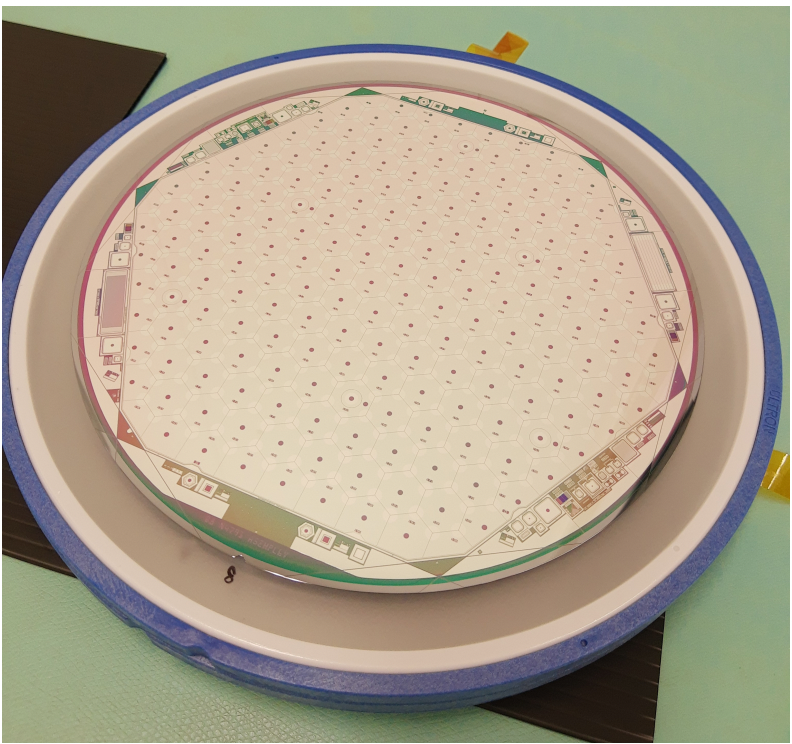
\includegraphics[width=.6\textwidth]{plots/LDsensors.png}
            \caption{LD sensors}
        \end{figure}
        \column{.5\textwidth}
        \begin{figure}
            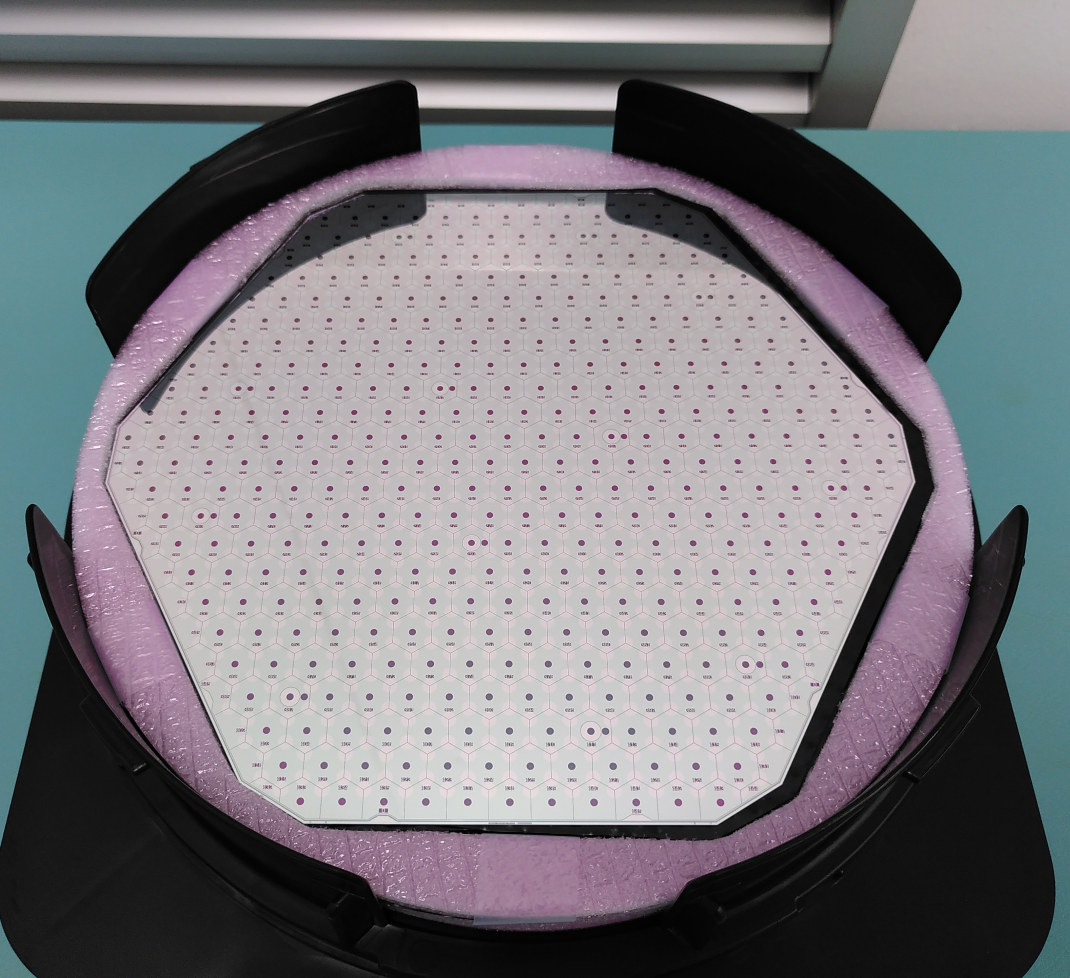
\includegraphics[width=.6\textwidth]{plots/HDsensors.png}
            \caption{HD sensors}
        \end{figure}
    \end{columns}

\end{frame}

\begin{frame}{Measurement Setup: PM8 and ALPS}
  \begin{columns}[b]
    \column{.5\textwidth}
      \begin{figure}
          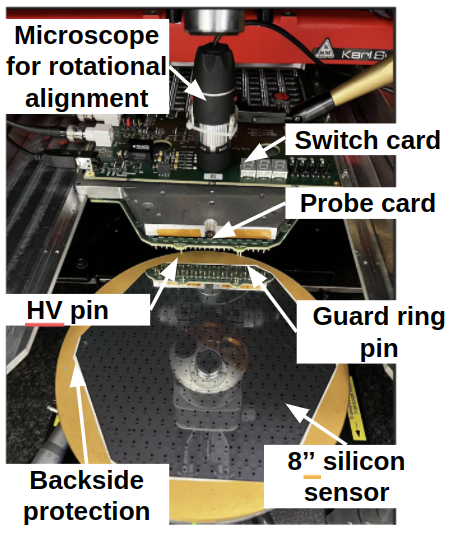
\includegraphics[width=.65\textwidth]{plots/PM8_description.png}
          \caption{PM8}
      \end{figure}
    \column{.5\textwidth}
      \begin{figure}
          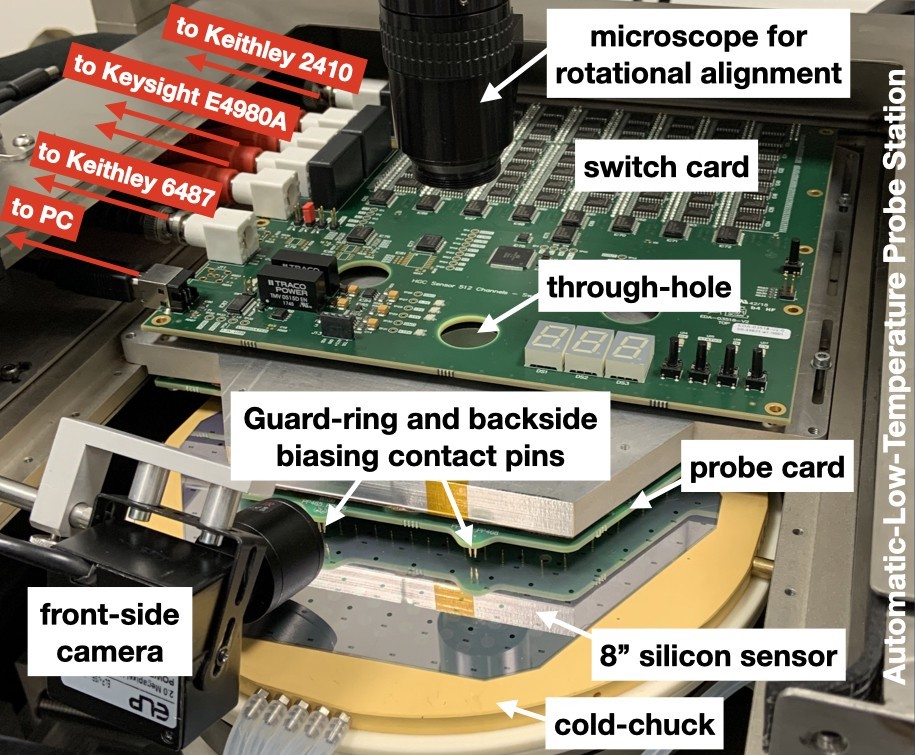
\includegraphics[width=.65\textwidth]{plots/ALPS_setup.png}
          \caption{ALPS}
      \end{figure}
  \end{columns}
    \begin{itemize}
        \small
        \item \alert{Pre-radiated} sensors
            \begin{itemize}
                \scriptsize
                \item  Room temperature; humidity: $ 40\% - 50\%$ ;  voltage up to \alert{-850V}
                \item Voltage provided through the HV pin to the frontside
            \end{itemize}
    \end{itemize}
\end{frame}




  

\section{IV Results}

\begin{frame}{IV grading criteria}
   \begin{itemize}
       \item \alert{Per-pad} characteristics (\alert{bad pad} definition)
            \begin{itemize}
                \item $ {I}_{600} > 100 nA $
                \item $ I600 > 10 nA  $  and $ I800 > 2.5 \times I600 $
                \item $ I600 <= 10 nA $  and $ I800 > 25 nA $
            \end{itemize}
       \item \alert{Global} characteristic
            \begin{itemize}
                \item I600 (normalised to 20 deg Celsius)$ <= 100 µA $ (integrated over all pads)
                \item $ I800 < 2.5 x I600 $
                \item Number of bad pads $ <= 8 $for full-sized sensors
                \item Allowed number of adjacent bad pads$ <= 2$
            \end{itemize}
   \end{itemize}

\end{frame}

\begin{frame}{IV results at CERN(HD) }
   \begin{columns}
        \column{.45\textwidth}
        \begin{figure}
            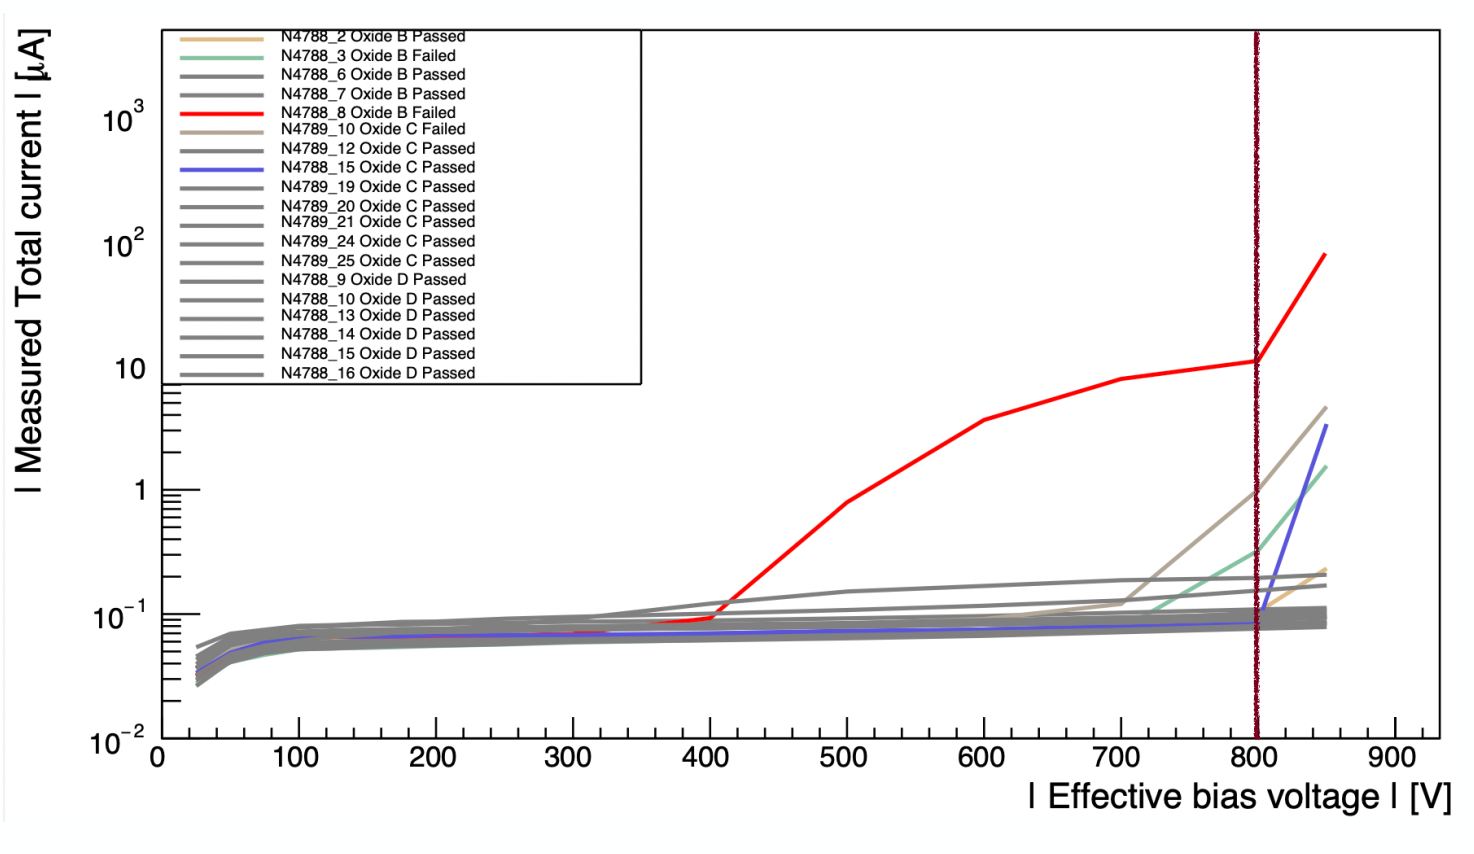
\includegraphics[width=1.0\textwidth]{plots/HD_totalIV.png}
            \caption{Total current of all 19 HD sensors}
        \end{figure}

        \column{.55\textwidth}
        \begin{figure}
            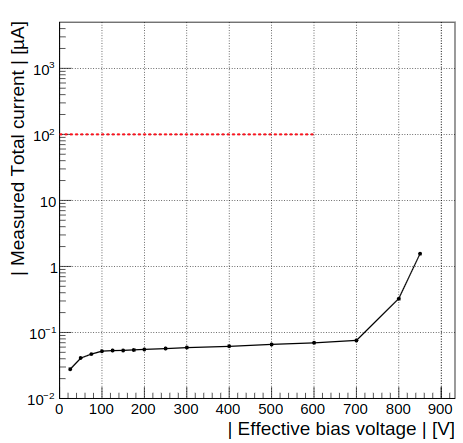
\includegraphics[width=0.6\textwidth]{plots/IV_Failed.png}
            \caption{One of the failed sensors}
        \end{figure}

    \end{columns}

    \begin{itemize}
        \item \alert{16 passed}, \alert{3 failed} for HD sensors
        \item Failing criteria:  $I_\text{800V, total} < 2.5 \times I_\text{600V, total}$
        \item Failing reason: one pad has high current readings
        \item Results of LD in backup
    \end{itemize}
\end{frame}


\begin{frame}{Comparison of IV results between HPK and CERN}
  \begin{figure}
    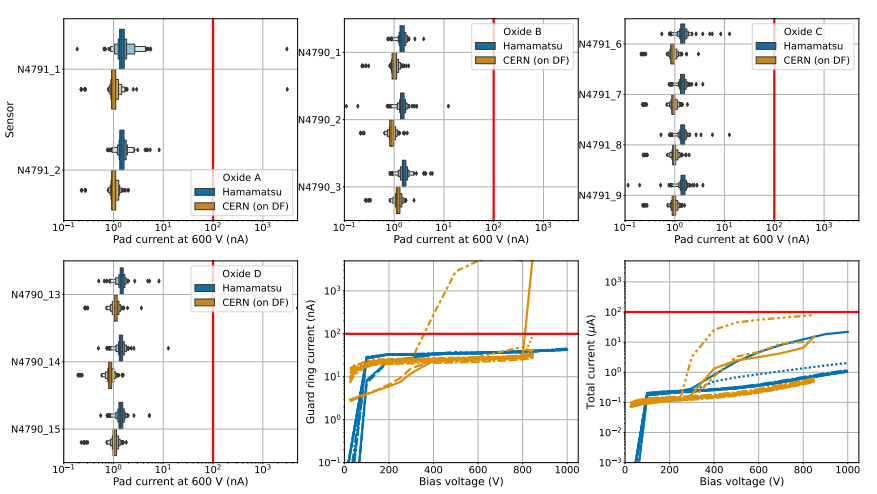
\includegraphics[width=.7\textwidth]{plots/IV_CERN_HPK_300um_cropped.png}
  \end{figure}
  \begin{itemize}
    \scriptsize
      \item In general, IV Measurement at CERN and that of HPK has \alert{good agreement}
      \item For \alert{guard ring}, CERN has slightly higher reading than HPK 
  \end{itemize}
\end{frame}

\begin{frame}{Summary for IV results}
    \begin{table}[htbp] %[h]
        \centering
        \footnotesize%Use \footnotesize for a 20% (linear) reduction in font size
        \setlength\tabcolsep{2pt}%Reduce the amount of intercolumn whitespace
        \resizebox{0.8\textwidth}{!}{% 
            \begin{tabular}{|c | c |c|c|} 
             \hline
             sensors  & passed sensors(CERN) & agreement with HPK & Source\\

             \hline
             HD (120um)  & \alert{16/19 } &  good agreement    &   \href{https://indico.cern.ch/event/1119831/contributions/4702464/attachments/2378225/4063679/Si\%20sensor\%20meeting.pdf}{\beamergotobutton{Link}} \\
             \hline
             LD (200um)&   \alert{12/12} & good agreement  &   \href{https://indico.cern.ch/event/1132823/contributions/4755812/attachments/2399581/4103704/LD\%20proto-A\%20sensors\%20200\%20um\%2C\%20ALPS\%20Winter\%202022.pdf}{\beamergotobutton{Link}} \\
             \hline
             LD (300um) &   \alert{14/14} & good agreement &   \href{https://indico.cern.ch/event/1085830/contributions/4565314/attachments/2344490/3998306/IVCV_recent_HGCal_prototype_sensors_Readiness_Review.pdf}{\beamergotobutton{Link}} \\
             \hline
            \end{tabular}
        }
        \caption{Summary for all protoA sensors}
        \end{table}   


    \begin{itemize}
        \item \alert{Majority} of sensors have \alert{good IV} results
        \item The reasons for failure were investigated
        % \item  \href{https://indico.cern.ch/event/1119831/contributions/4702464/attachments/2378225/4063679/Si%20sensor%20meeting.pdf}{links}
        
        
    \end{itemize}
\end{frame}


\section{CV Results}

\begin{frame}{Proto-A: example CV results}
  \begin{figure}
      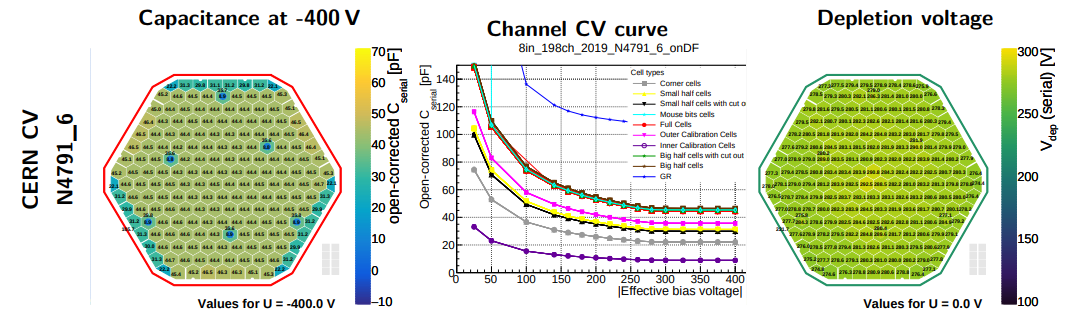
\includegraphics[width=1.0\textwidth]{plots/CV_example.png}    
  \end{figure}
  \begin{itemize}
    \item HexPlots as graphical representation of cell properties on the sensor
    \item CV curves
  \end{itemize}
\end{frame}

\begin{frame}{CV grading criteria}
  \begin{itemize}
      \item \alert{Global} characteristic from full hexagonal pads only
        \begin{itemize}
          \item Depletion voltage $ median(V_{dep}) $:
            \begin{itemize}
             \item $ < 370 V $ for thickness 300 um
             \item $ < 160 V $ for thickness 200 um
             \item $ < 70 V $ for thickness 120 um  
            \end{itemize}
          \item Depletion voltage uniformity ($ IQR_{68\%}(V_{dep}) $):
            \begin{itemize}
              \item $< 0.1 * median(V_{dep})$
            \end{itemize}
          \item Thickness uniformity ${\Delta} thickness$:
            \begin{itemize}
              \item $< +/- 10um $
            \end{itemize}
        \end{itemize}
  \end{itemize}
\end{frame}

\begin{frame}{LD 300 um, CV results: HPK and CERN (on DF)}
    \begin{figure}
        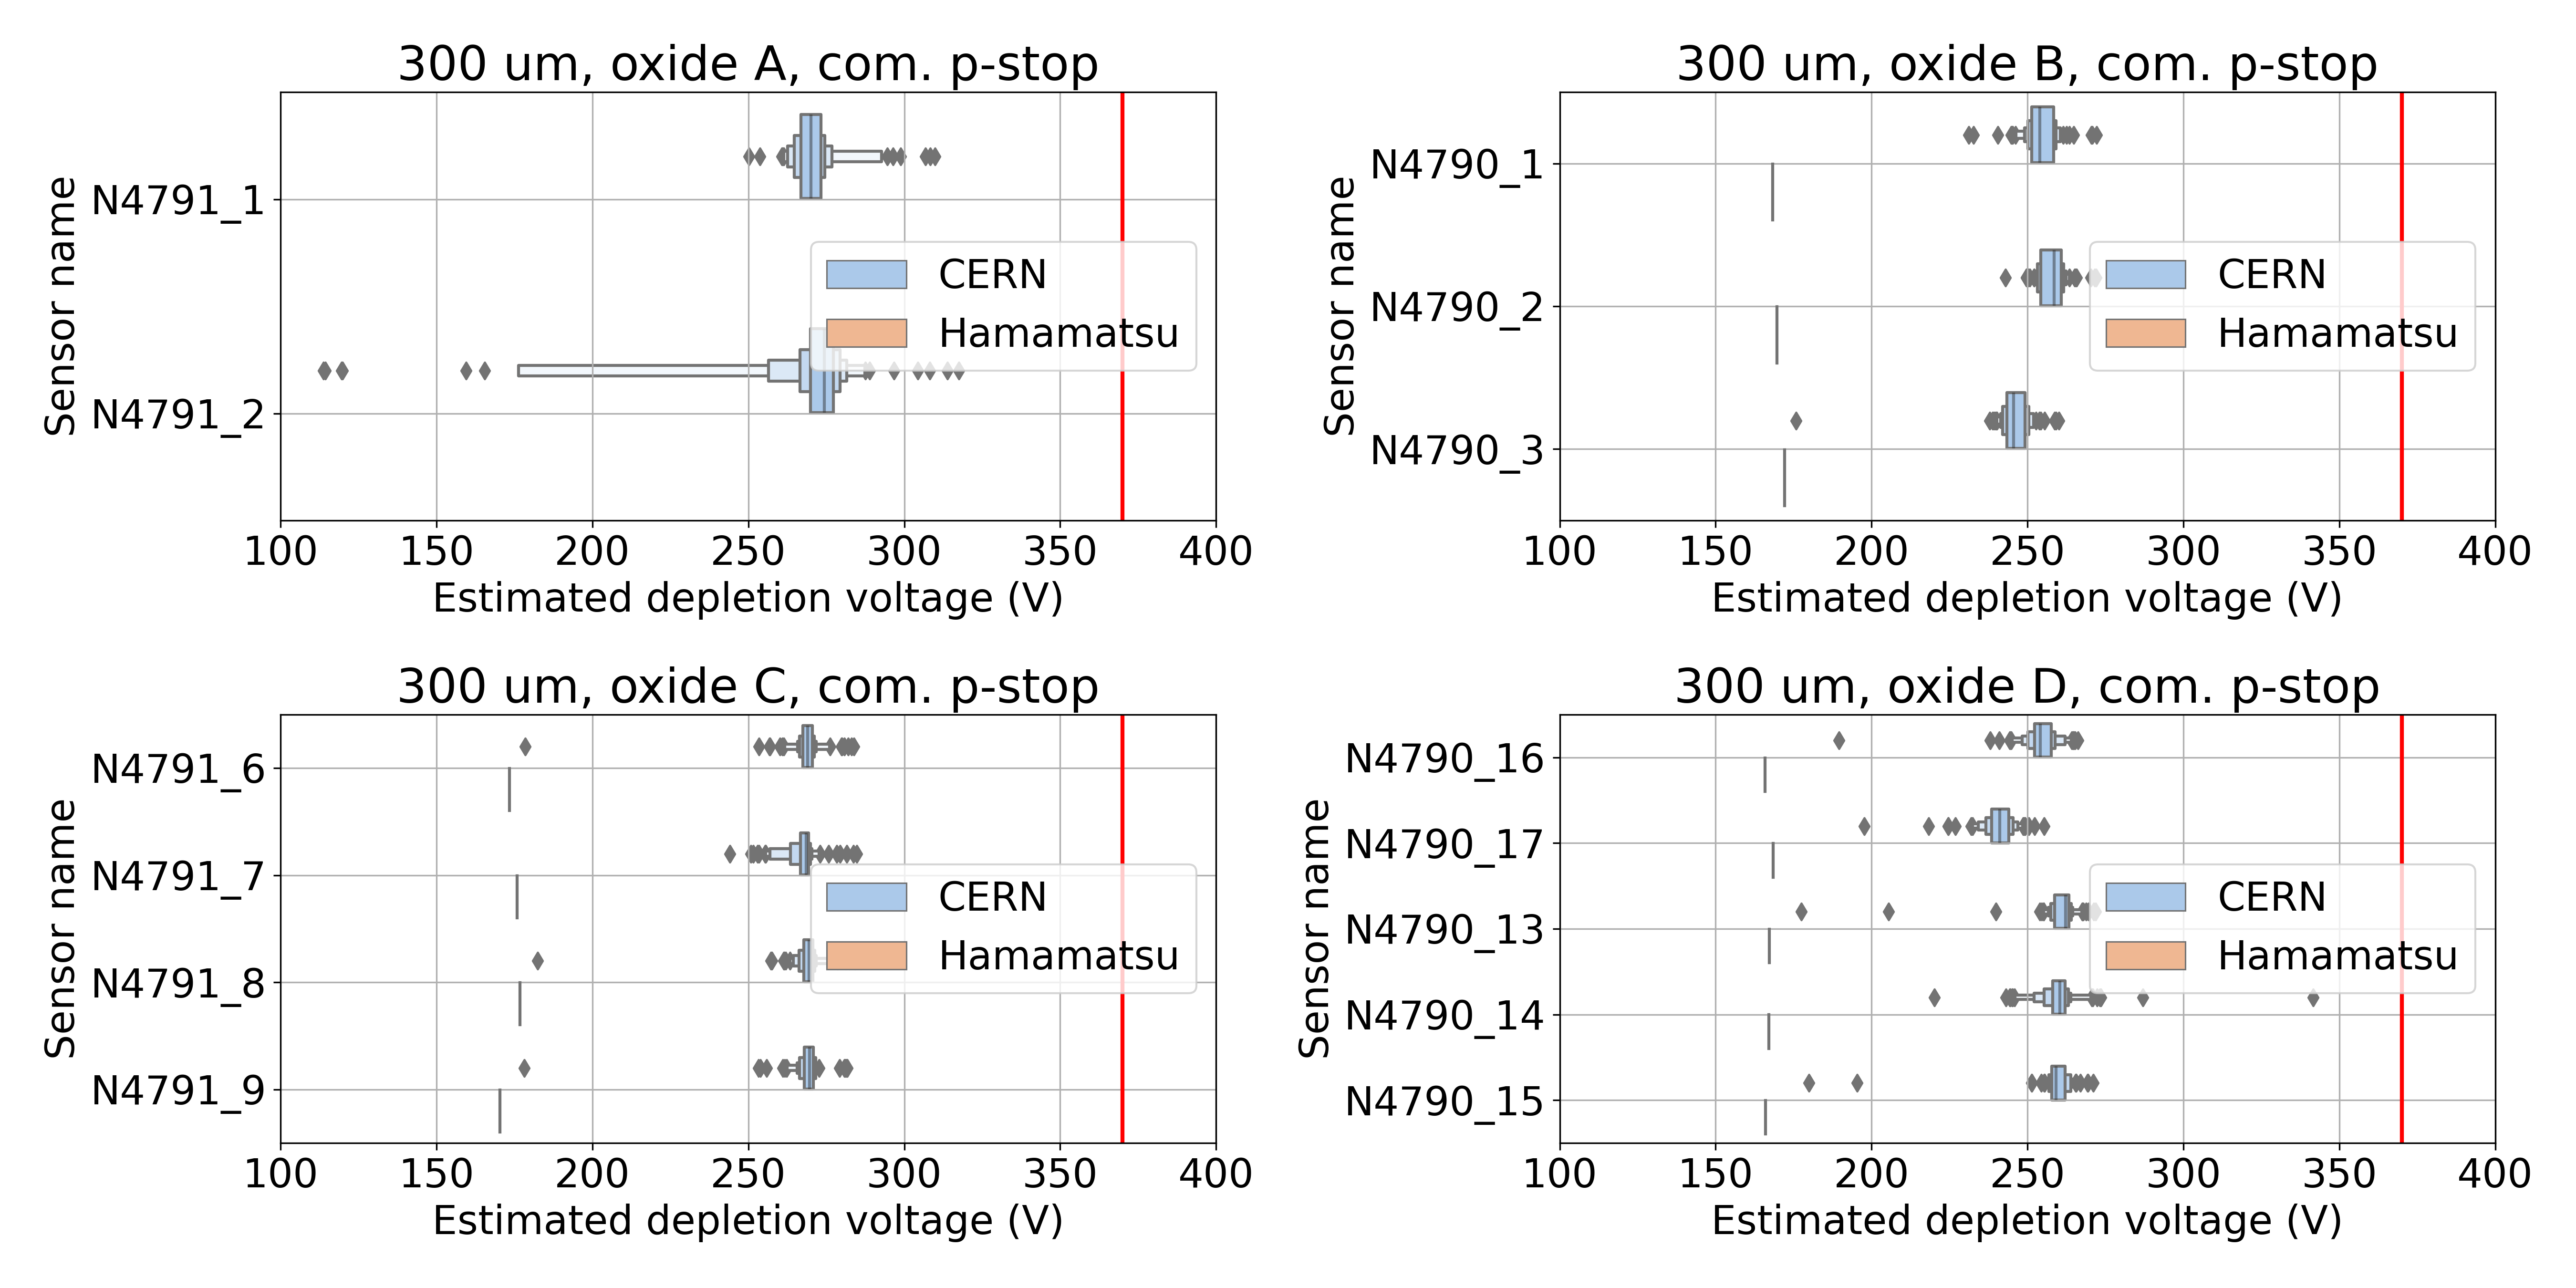
\includegraphics[width=.9\textwidth]{plots/CV_ComparisonHPKCERN_300um_All.png}    
    \end{figure}
  \href{https://indico.cern.ch/event/1085830/contributions/4565314/attachments/2344490/3998306/IVCV_recent_HGCal_prototype_sensors_Readiness_Review.pdf}{\beamergotobutton{Proto-A, 300 um}}
\end{frame}

% \begin{frame}{HD 120 um, depletion voltage fit fails for some cells}
%   \begin{columns}
%     \column{.5\textwidth}
%     \begin{figure}
%       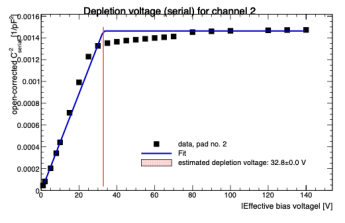
\includegraphics[width=.55\textwidth]{plots/CV_Fit_just_figures1.png}
%       %\caption{Successful fit: most cells}
%     \end{figure}
%     \column{.5\textwidth}
%     \begin{figure}
%       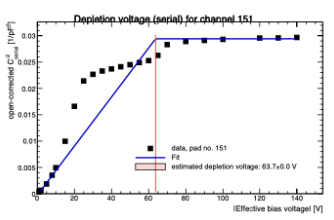
\includegraphics[width=.55\textwidth]{plots/CV_Fit_just_figures2.png}
%       \caption{Strange fit: calibration cells and edge cells}
%     \end{figure}
%     \begin{figure}
%       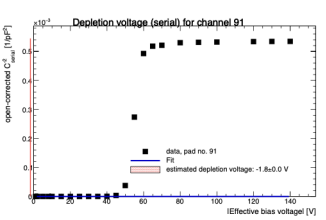
\includegraphics[width=.55\textwidth]{plots/CV_Fit_just_figures3.png}
%       \caption{Failed fit: random cells}
%     \end{figure}

% \end{columns}

%   \begin{figure}
    
%   \end{figure}
%   \href{https://indico.cern.ch/event/1119831/contributions/4702464/attachments/2378225/4063679/Si\%20sensor\%20meeting.pdf}{\beamergotobutton{Proto-A, 120 um}}

% \end{frame}

\begin{frame}{HD 120 um, depletion voltage fit fails for some cells}
  \begin{columns}
    \column{.5\textwidth}
    \begin{figure}
      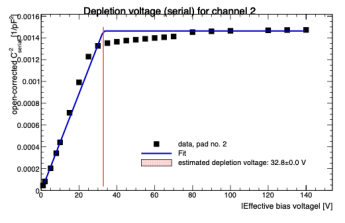
\includegraphics[width=.55\textwidth]{plots/CV_Fit_just_figures1.png}
      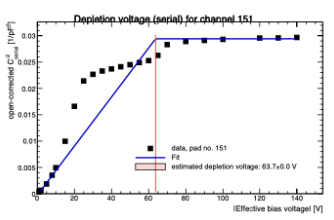
\includegraphics[width=.55\textwidth]{plots/CV_Fit_just_figures2.png}
      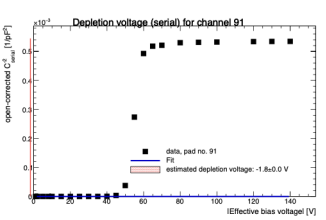
\includegraphics[width=.55\textwidth]{plots/CV_Fit_just_figures3.png}
      %\caption{Successful fit: most cells}
    \end{figure}
    \column{.5\textwidth}

    \begin{itemize}
      \item Successful fit: for most cells of the sensors
      \item Strange fit: calibration cells and edge cells, same cells for all the sensors
      \item Failed fit: random cells for the sensors
    \end{itemize}
    \href{https://indico.cern.ch/event/1119831/contributions/4702464/attachments/2378225/4063679/Si\%20sensor\%20meeting.pdf}{\beamergotobutton{Proto-A, 120 um}}


\end{columns}

\end{frame}


\begin{frame}{Summary for CV results}
  \begin{table}[htbp] %[h]
      \centering
      \footnotesize%Use \footnotesize for a 20% (linear) reduction in font size
      \setlength\tabcolsep{2pt}%Reduce the amount of intercolumn whitespace
      \resizebox{0.8\textwidth}{!}{% 
          \begin{tabular}{|c | c |c|c|} 
           \hline
           sensors  & passed sensors(CERN) & agreement with HPK \\

           \hline
           HD (120um)  & \alert{13/13 }               & good agreement &   \href{https://indico.cern.ch/event/1119831/contributions/4702464/attachments/2378225/4063679/Si\%20sensor\%20meeting.pdf}{\beamergotobutton{Link}} \\
           \hline
           LD (200um)&   \alert{5/5} & good agreement &   \href{https://indico.cern.ch/event/1132823/contributions/4755812/attachments/2399581/4103704/LD\%20proto-A\%20sensors\%20200\%20um\%2C\%20ALPS\%20Winter\%202022.pdf}{\beamergotobutton{Link}} \\
           \hline
           LD (300um) &   \alert{14/14} & good agreement &   \href{https://indico.cern.ch/event/1085830/contributions/4565314/attachments/2344490/3998306/IVCV_recent_HGCal_prototype_sensors_Readiness_Review.pdf}{\beamergotobutton{Link}} \\
           \hline
          \end{tabular}
      }
      \caption{Summary for all protoA sensors}
      \end{table}   


  \begin{itemize}
      \item \alert{All} sensors have \alert{passed} CV grading      
      
  \end{itemize}
\end{frame}

\section{Additional Measurements}


\begin{frame}{Longterm Leakage current stability}
  \begin{figure}
    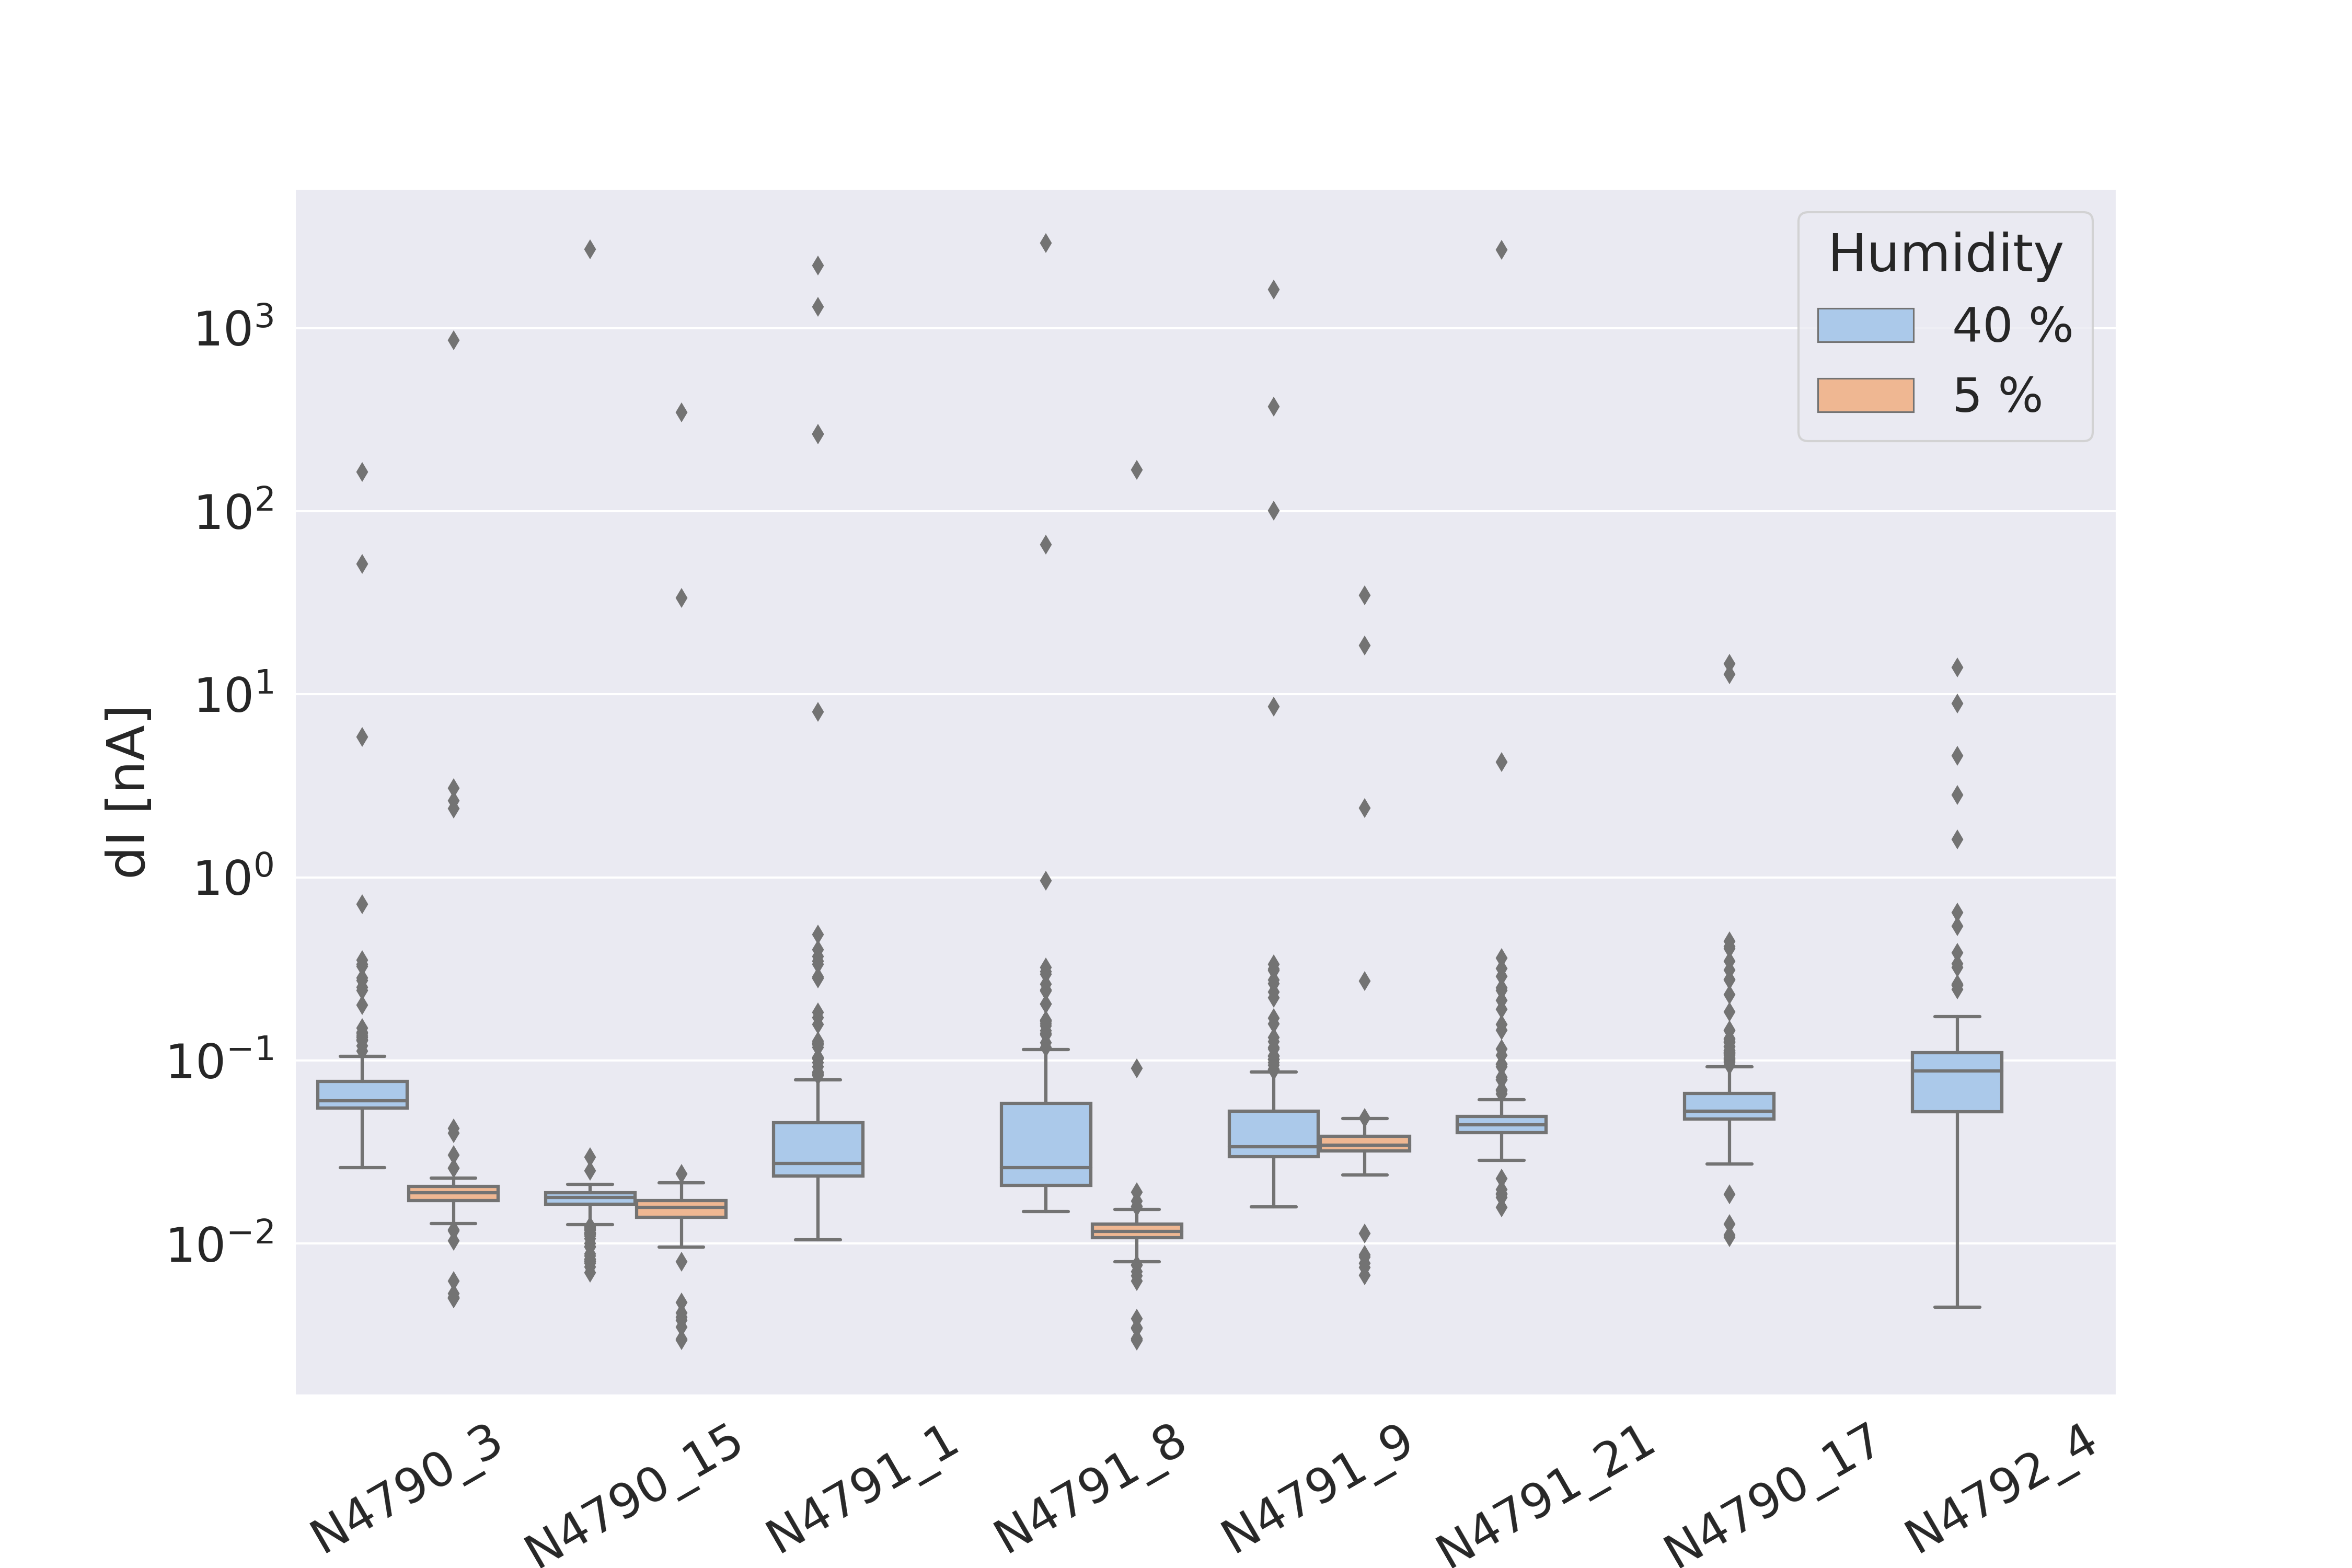
\includegraphics[width=.8\textwidth]{plots/RangesForCurrentVariationsDryAir.png}
  \end{figure}
  \href{https://indico.cern.ch/event/1121372/contributions/4708329/attachments/2382634/4071804/Longterm_Leakage_Current_Measurements.pdf}{\beamergotobutton{Longterm Current}}
\end{frame}

\begin{frame}{Dicing Frame removal at CERN}
  \begin{columns}
    \column{.5\textwidth}
    \begin{figure}
      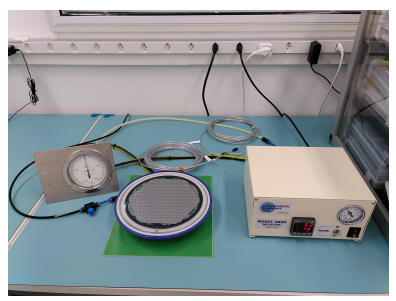
\includegraphics[width=1.0\textwidth]{plots/DF_removal_Picture.png}
      \caption{Dicing Frame Removal Process at CERN}
    \end{figure}

    \column{.55\textwidth}
    \begin{itemize}
      \item Process Parameters:
      \begin{itemize}
        \item UV illumination
        \item Temperature: $50  ^oC$
        \item 600 mbar vacuum
      \end{itemize}
      \item Result:
      \begin{itemize}
        \item For the 300 um sensors 6 of previously 11 good sensors failed the IV requirements
        \item 120 um and 200 um sensors were delivered off-DF
      \end{itemize}
    \end{itemize}

\end{columns}

\begin{figure}
\end{figure} 
  \href{https://indico.cern.ch/event/1085830/contributions/4565314/attachments/2344490/3998306/IVCV_recent_HGCal_prototype_sensors_Readiness_Review.pdf}{\beamergotobutton{Dicing Frame (Slide 24)}}
\end{frame}


\begin{frame}{Summary}
  \begin{itemize}
    % \scriptsize
    \item Majority of sensors have good IV results
    \item CV results are good for all proto-A sensors
    \item Longterm leakage current instability can be observed  for some channels
    \item No discharges has been observed for proto A sensors
    % \item Test throughput 20 sensors per week
    % \item Shortage of LCR meters problem resolved
  \end{itemize}
\end{frame}

\appendix

\begin{frame}{Backup}
	\center
	\huge
	Backup slides
\end{frame}

\begin{frame}{Sensor list: HD}
   \begin{figure}
       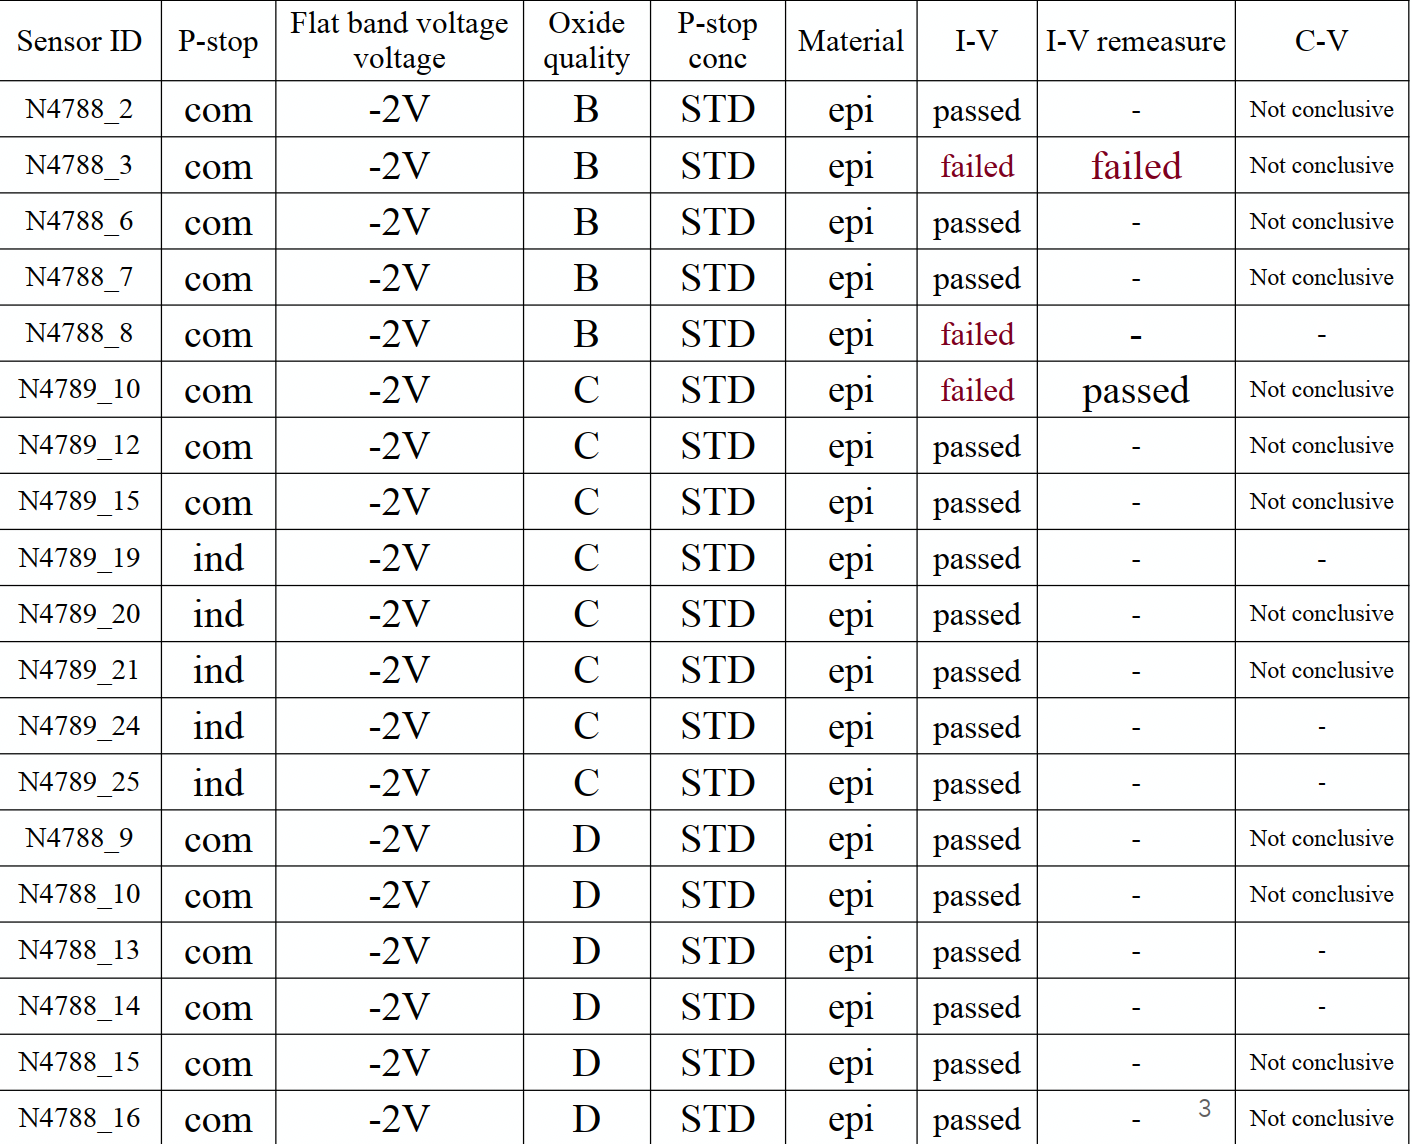
\includegraphics[width=.8\textwidth]{plots/PM8_sensorList.png}
   \end{figure} 
\end{frame}


\begin{frame}{Sensor list: LD}
   \begin{figure}
       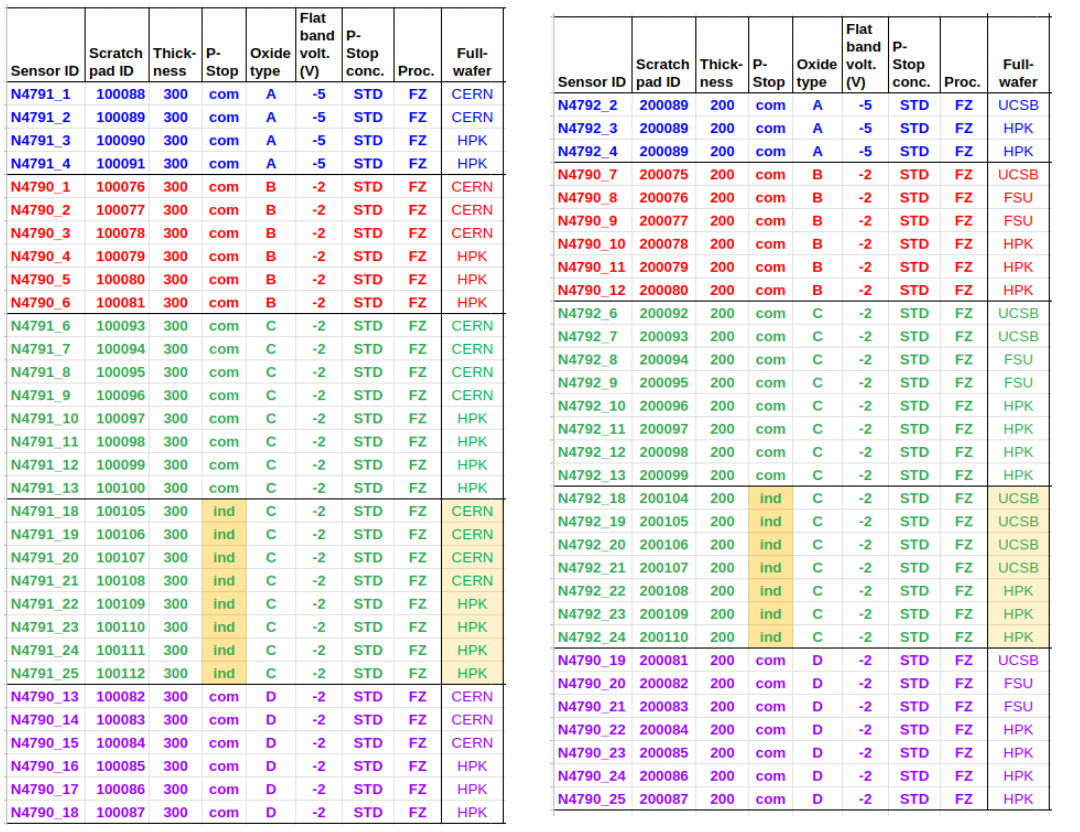
\includegraphics[width=.8\textwidth]{plots/Fall_2021_sensorList.png}
   \end{figure} 
\end{frame}


\begin{frame}{Proto-A, 120 um, CV results: HPK and CERN}
  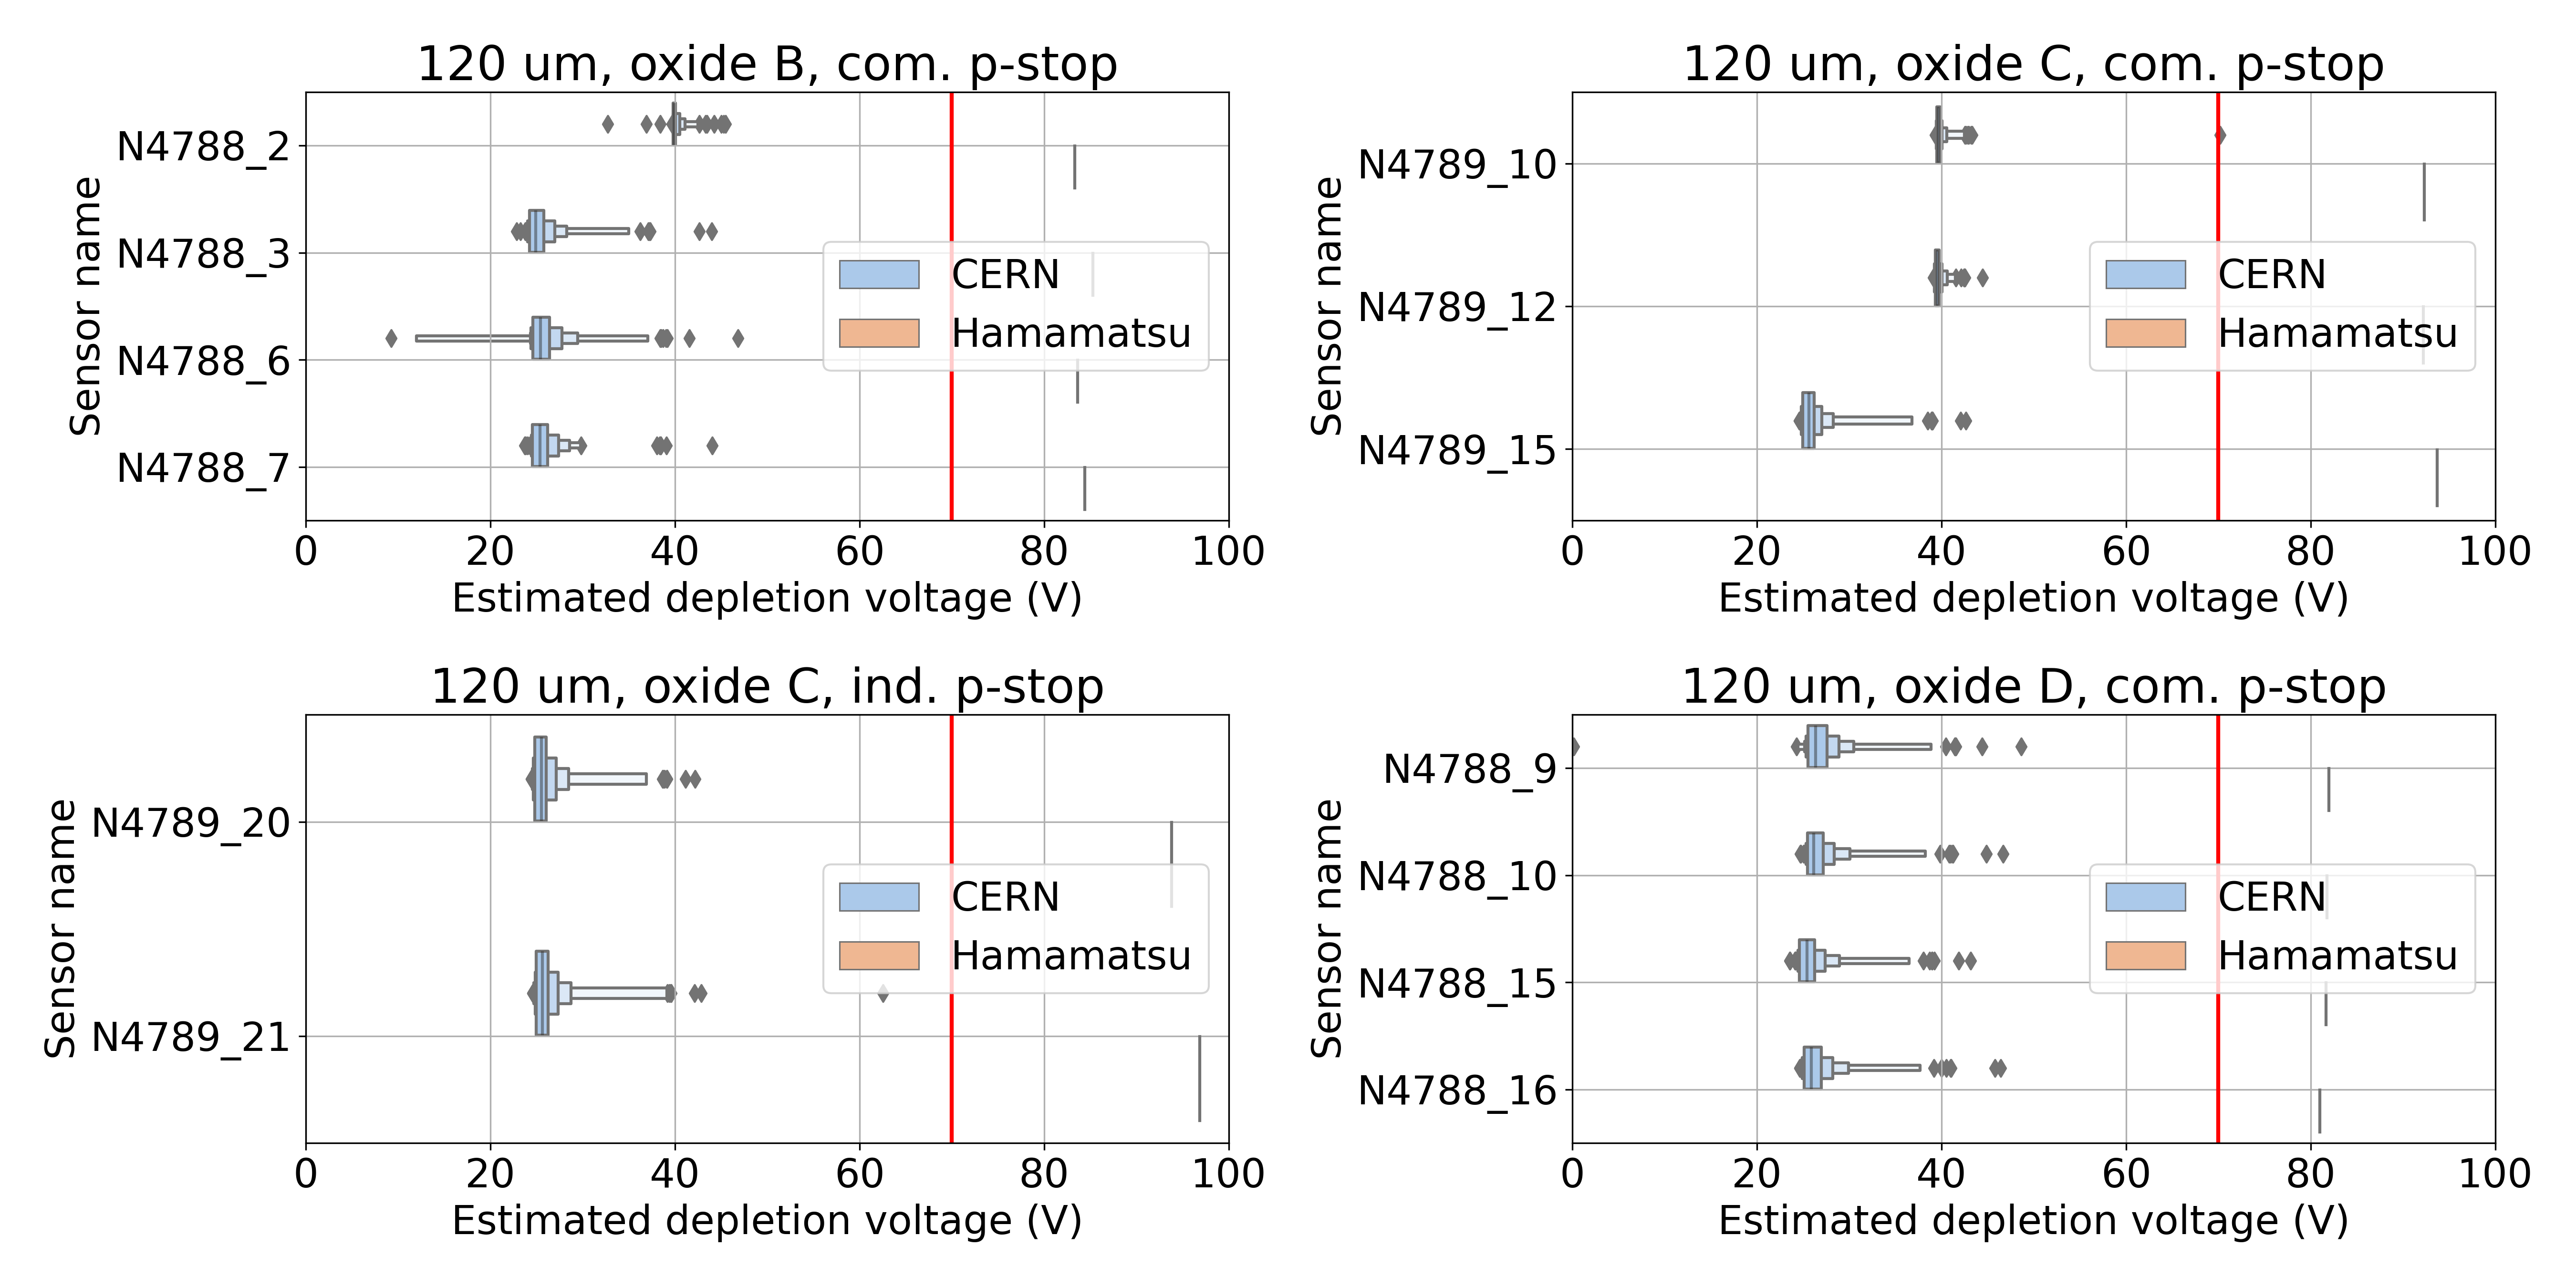
\includegraphics[width=.8\textwidth]{plots/CV_ComparisonHPKCERN_120um.png}
  \begin{block}{}
    \begin{itemize}
      % \scriptsize
      \item Hamamatsu results are outside the treshhold. CERN results are good.
      \item Hamamatsu measures one diode, while CERN measures all channels.
      \item Hamamatsu measures on Dicing Frame, which CERN off Dicing Frame.
    \end{itemize}
  \end{block}
\end{frame}
\begin{frame}{Proto-A, 200 um, CV results: HPK and CERN (on DF)}
  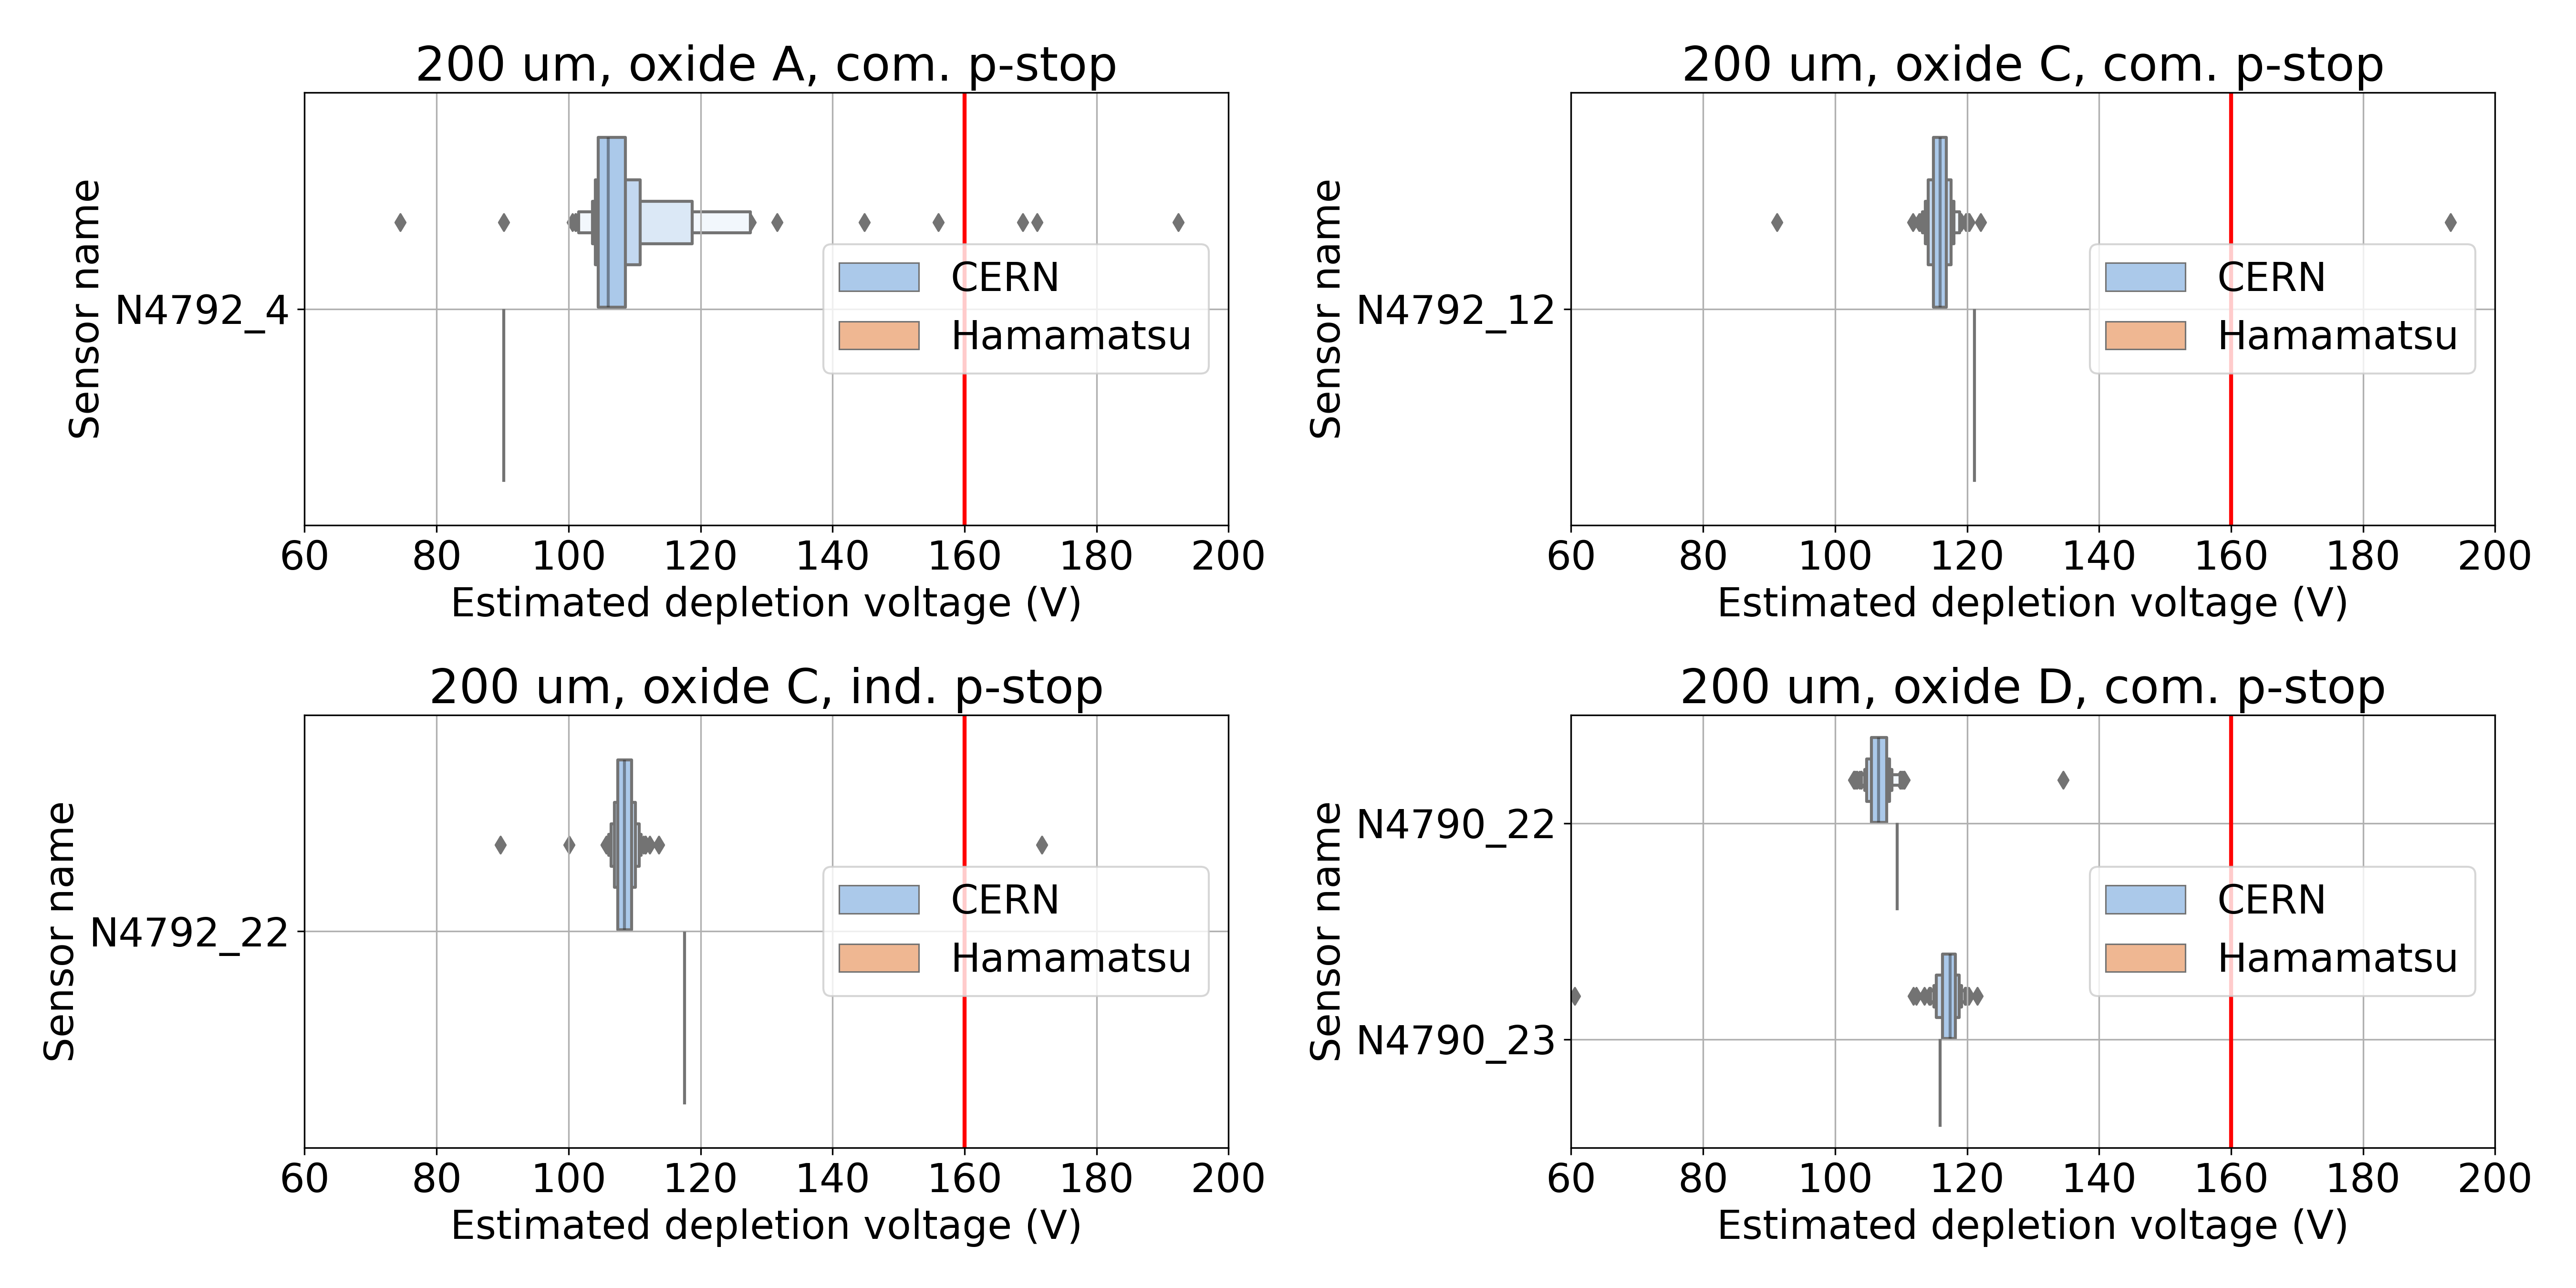
\includegraphics[width=.9\textwidth]{plots/CV_ComparisonHPK_200um.png}
  \href{https://indico.cern.ch/event/1132823/contributions/4755812/attachments/2399581/4103704/LD\%20proto-A\%20sensors\%20200\%20um\%2C\%20ALPS\%20Winter\%202022.pdf}{\beamergotobutton{Proto-A, 200 um}}
\end{frame}

\begin{frame}{Proto-A, 200 um, CV grading (all passed)}
  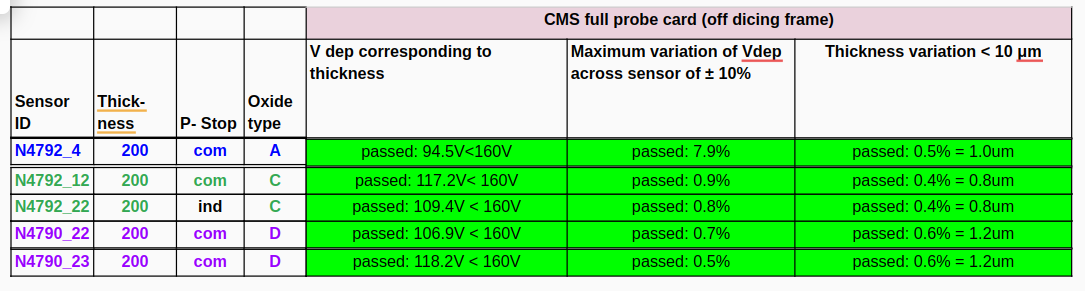
\includegraphics[width=.7\textwidth]{plots/CV_grading_200um.png}
\end{frame}

\begin{frame}{Proto-A, 300 um, CV grading comparison}
  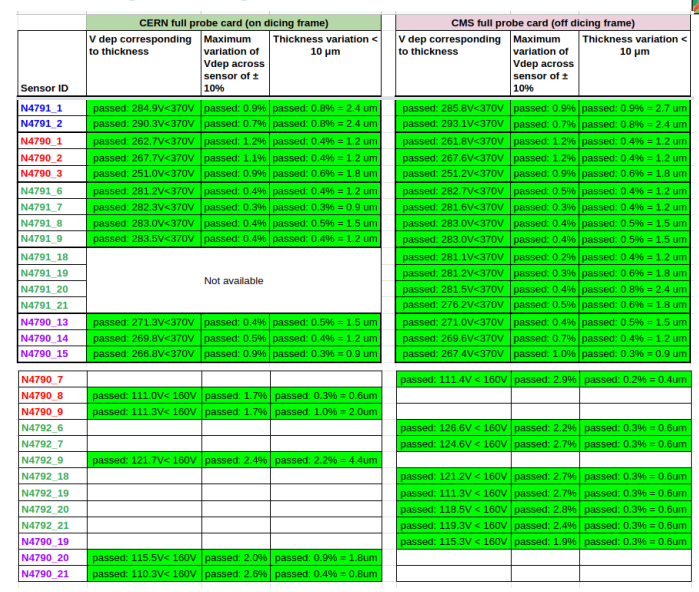
\includegraphics[width=.7\textwidth]{plots/CV_grading_300um.png}
\end{frame}

\begin{frame}{Proto-A Batch 2, 300 um, CV results: HPK and CERN (on DF)}
  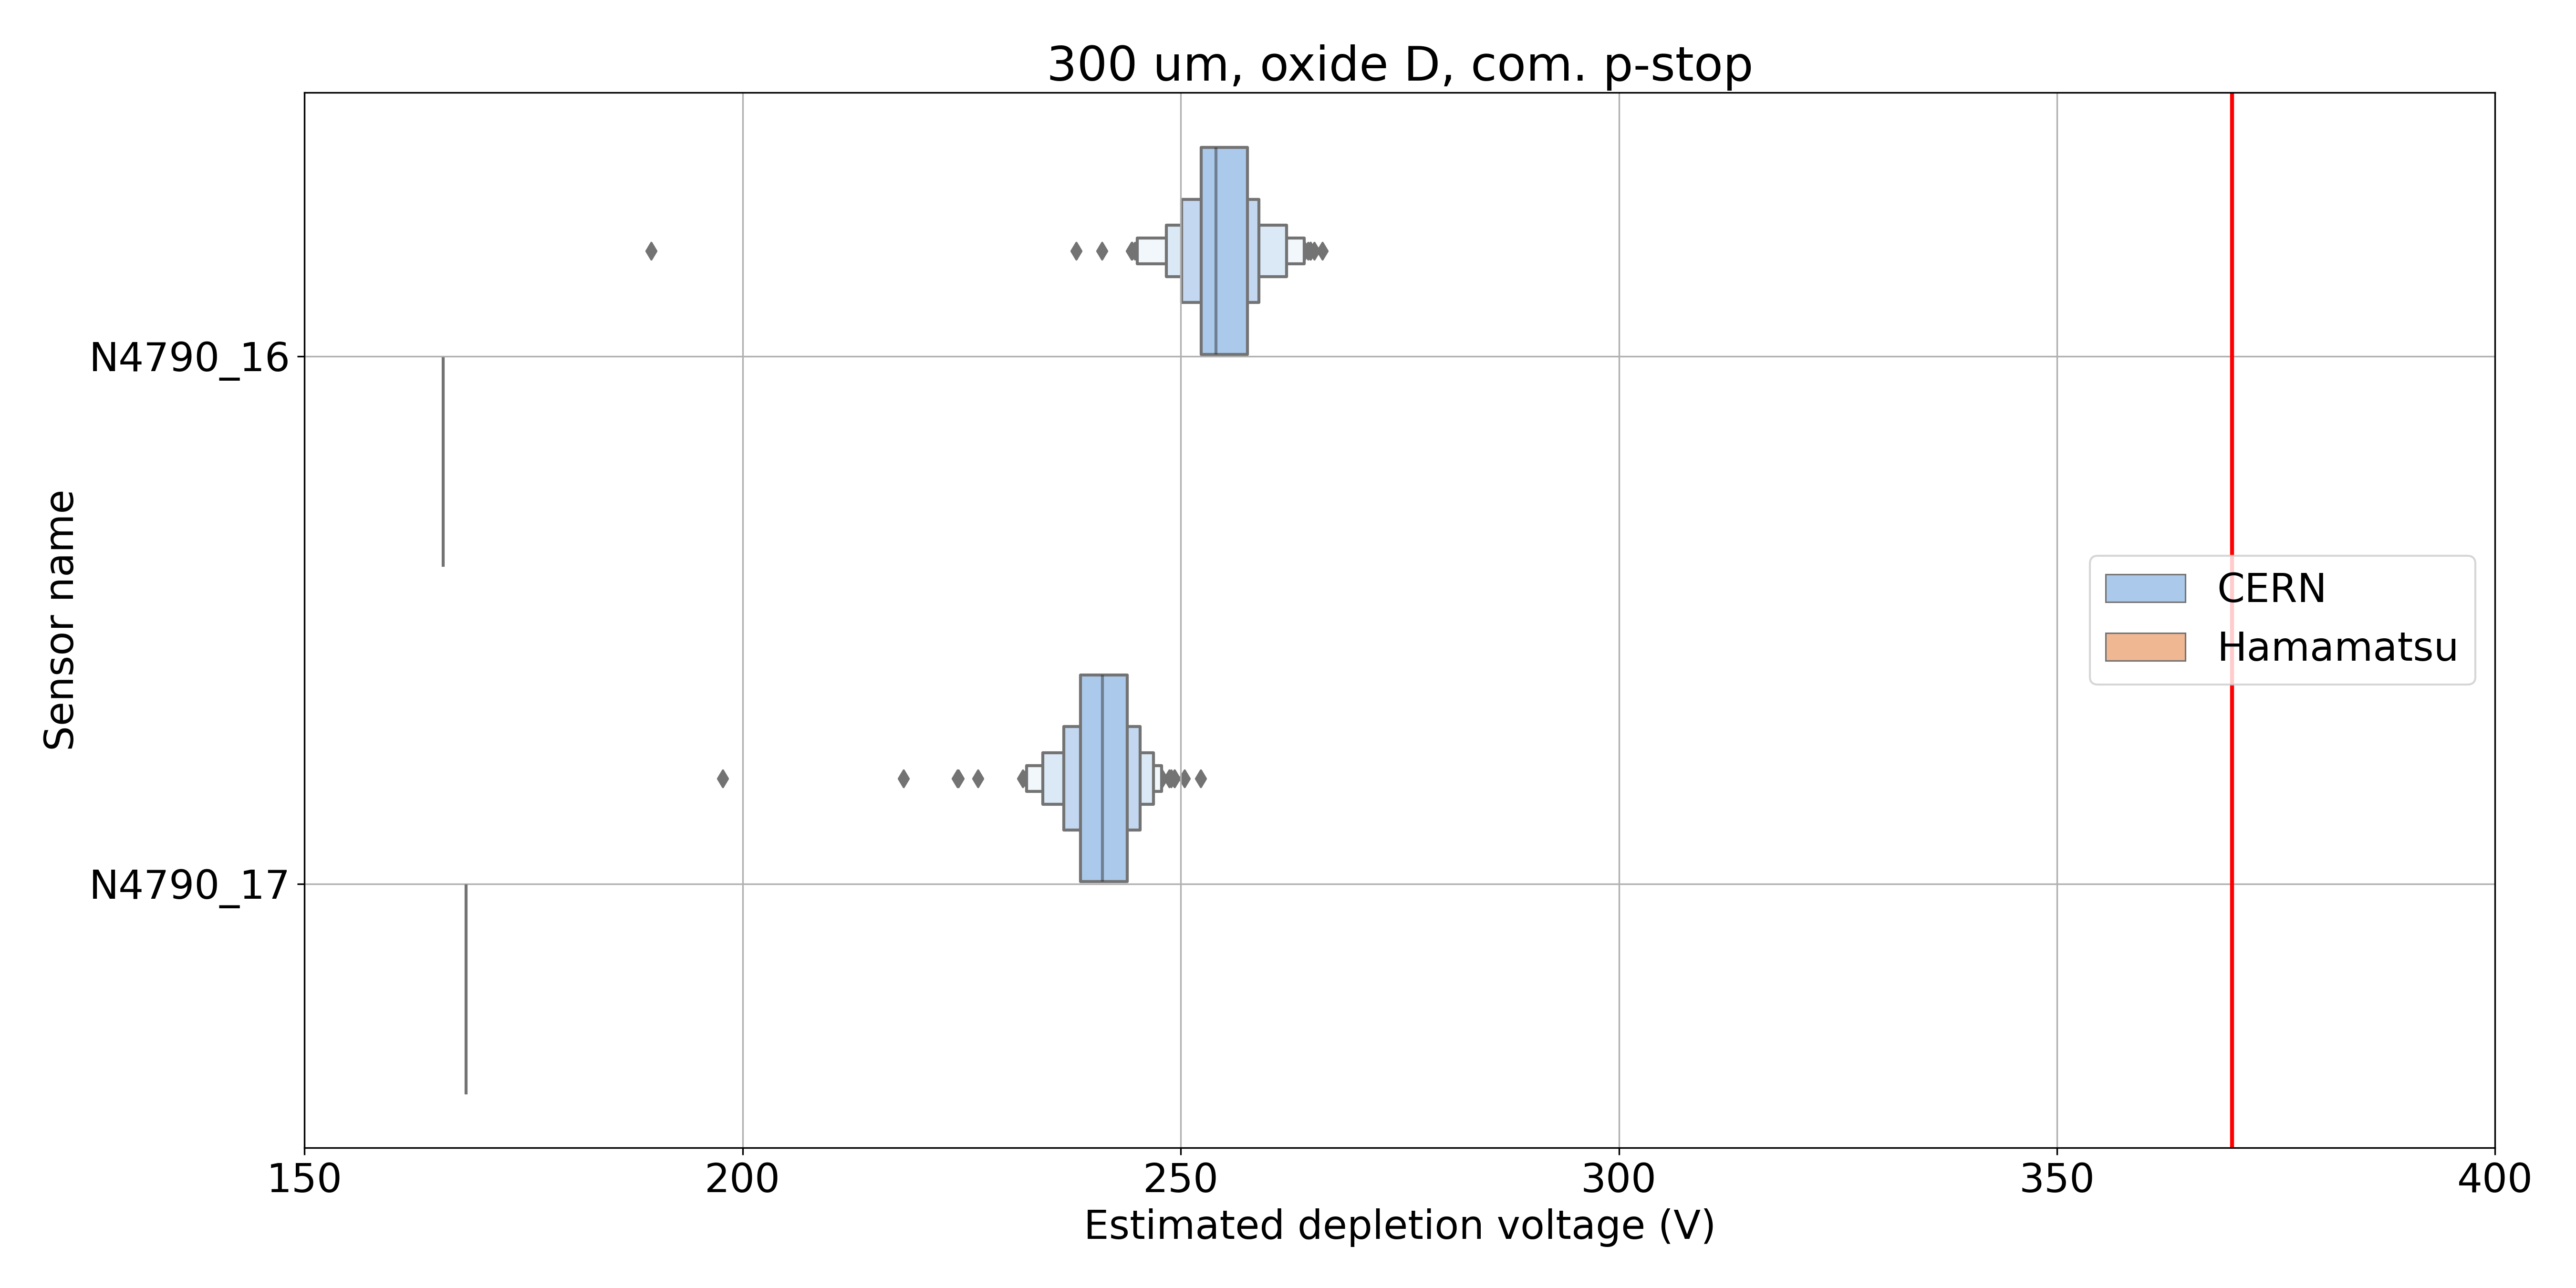
\includegraphics[width=.8\textwidth]{plots/CV_ComparisonHPK_300um.png}
\end{frame}

\begin{frame}{Proto-A, Batch 2, 300 um, CV grading comparison}
  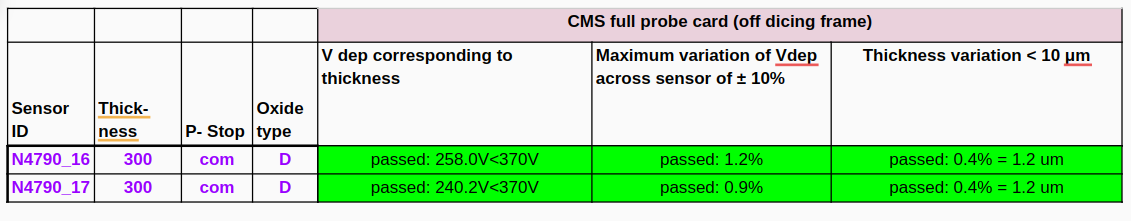
\includegraphics[width=.7\textwidth]{plots/CV_grading_300um_2.png}
\end{frame}

\begin{frame}{Proto-A, 120 um, failed fits, cell distribution}
  \begin{figure}
    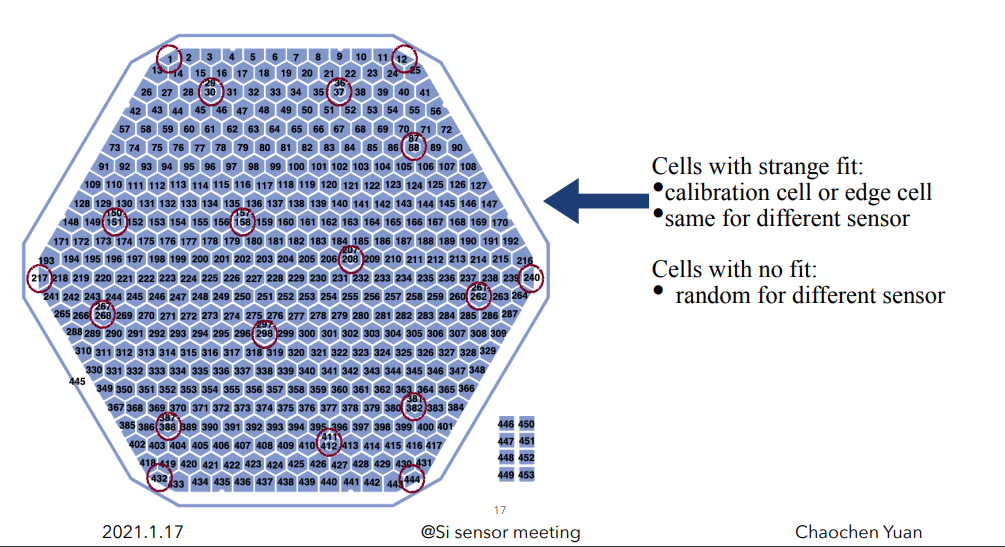
\includegraphics[width=.9\textwidth]{plots/CV_Fit_Distribution.png}
  \end{figure}
\end{frame}

\begin{frame}{Longterm Leakage current stability, sensors}
  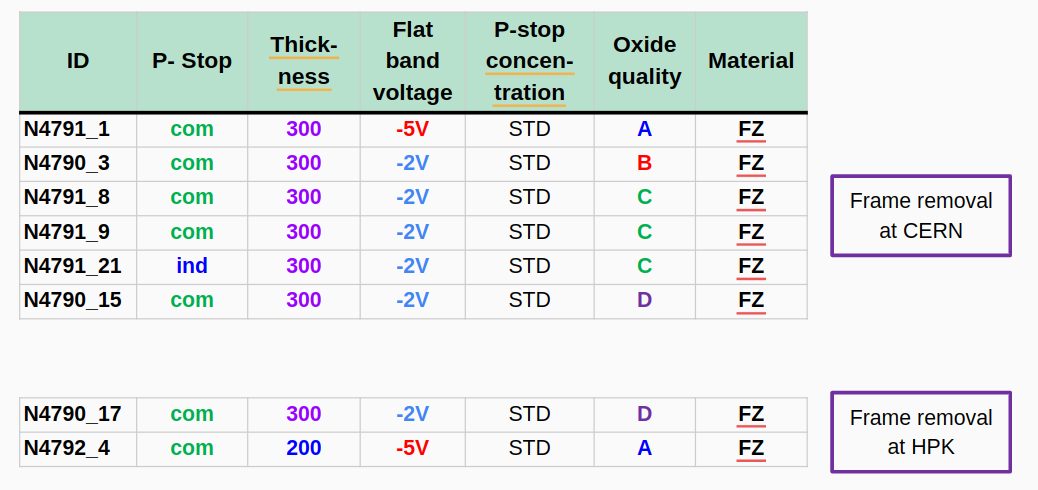
\includegraphics[width=.9\textwidth]{plots/Longterm_sensors.png}
\end{frame}

\begin{frame}{Longterm Leakage current stability}
  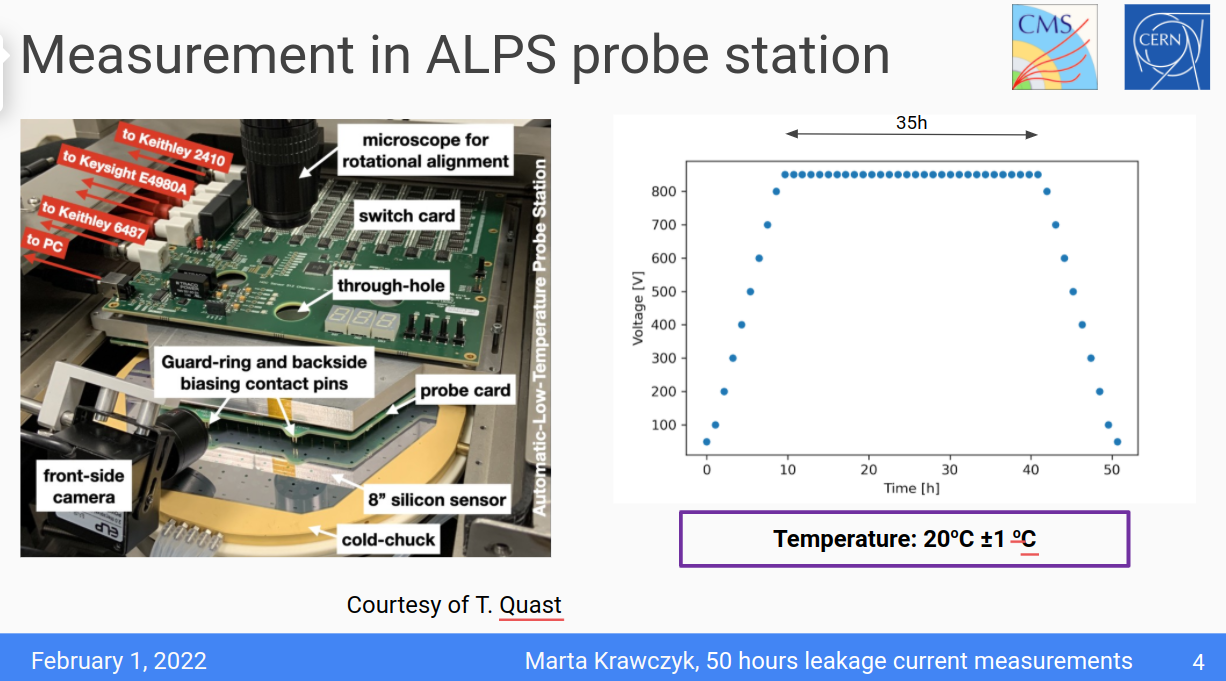
\includegraphics[width=.7\textwidth]{plots/Longterm_process.png}
\end{frame}

\begin{frame}{Proto-A: example IV+CV results}
    \begin{figure}
  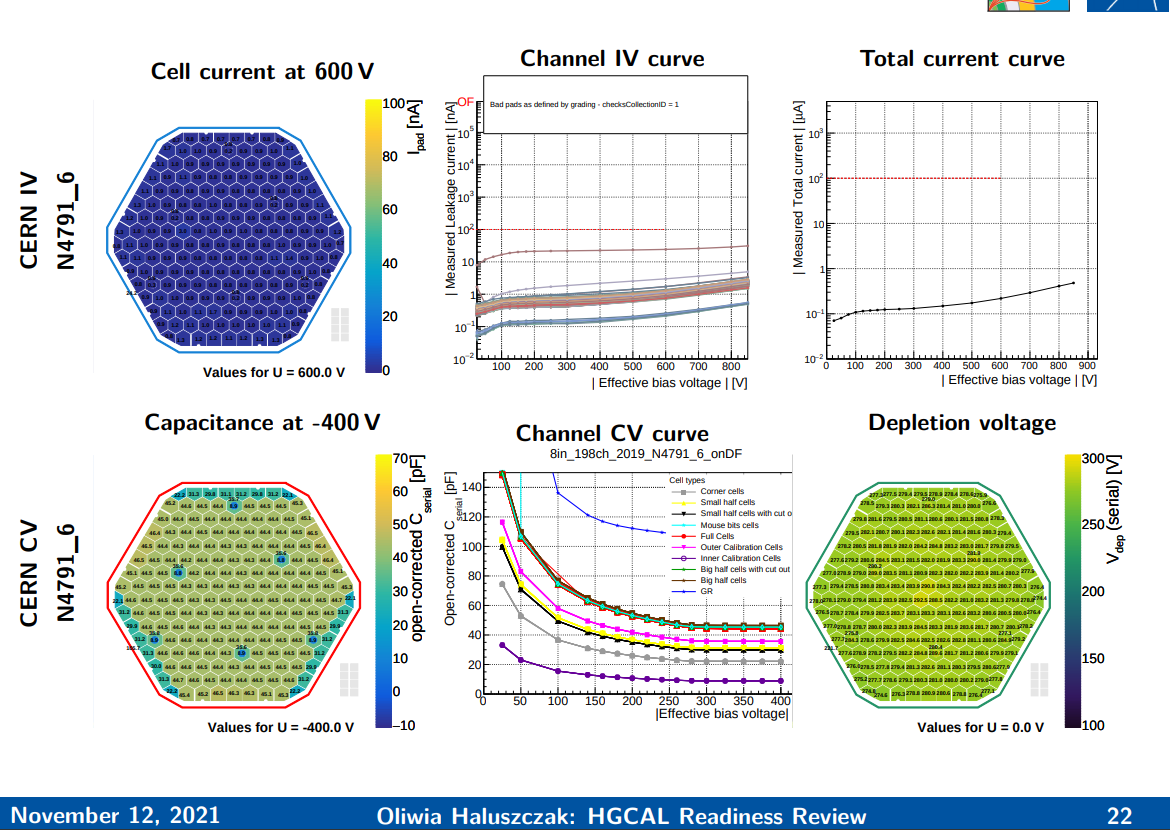
\includegraphics[width=.8\textwidth]{plots/IV_CV_example.png}
        
    \end{figure}
\end{frame}


%\begin{frame}
%\frametitle{Sample frame title}
%
%In this slide, some important text will be
%\alert{highlighted} because it's important.
%Please, don't abuse it.
%
%\begin{block}{Remark}
%Sample text
%\end{block}
%
%\begin{alertblock}{Important theorem}
%Sample text in red box
%\end{alertblock}
%
%\begin{examples}
%Sample text in green box. The title of the block is ``Examples".
%\end{examples}
%\end{frame}
%
%\begin{frame}{Make Titles Informative.}
%  You can create overlays\dots
%  \begin{itemize}
%  \item using the \texttt{pause} command:
%    \begin{itemize}
%    \item
%      First item.
%      \pause
%    \item    
%      Second item.
%    \end{itemize}
%  \item
%    using overlay specifications:
%    \begin{itemize}
%    \item<3->
%      First item.
%    \item<4->
%      Second item.
%    \end{itemize}
%  \item
%    using the general \texttt{uncover} command:
%    \begin{itemize}
%      \uncover<5->{\item
%        First item.}
%      \uncover<6->{\item
%        Second item.}
%    \end{itemize}
%  \end{itemize}
%\end{frame}
%
%
%% All of the following is optional and typically not needed. 
%\appendix
%\section<presentation>*{\appendixname}
%\subsection<presentation>*{For Further Reading}
%
%\begin{frame}[allowframebreaks]
%  \frametitle<presentation>{For Further Reading}
%    
%  \begin{thebibliography}{10}
%    
%  \beamertemplatebookbibitems
%  % Start with overview books.
%
%  \bibitem{Author1990}
%    A.~Author.
%    \newblock {\em Handbook of Everything}.
%    \newblock Some Press, 1990.
% 
%    
%  \beamertemplatearticlebibitems
%  % Followed by interesting articles. Keep the list short. 
%
%  \bibitem{Someone2000}
%    S.~Someone.
%    \newblock On this and that.
%    \newblock {\em Journal of This and That}, 2(1):50--100,
%    2000.
%  \end{thebibliography}
%\end{frame}

\end{document}


